%!TEX root = ../thesis.tex
%*******************************************************************************
%****************************** Third Chapter **********************************
%*******************************************************************************
\chapter{Fabrication and Characterisation Methodologies}


\section[Fabrication Procedure]{Fabrication Procedure}

It is imperative that the capability of the devices to exhibit distinct and stable state-dependent conductance changes is demonstrated prior to the design of novel neuromorphic systems. These conductance changes are modelled in neuronal spiking systems. \\

\noindent The present chapter thus provides a detailed account of the experimental methodology employed in this study, alongside a comprehensive presentation of the results obtained from the experiments. The aforementioned devices have been demonstrated to exhibit a variety of non-volatile switching properties. The measurements are focused on the electrical characteristics and switching mechanism of the samples. \\

\noindent The devices investigated in this thesis were developed by the Electronic Materials and Devices group in the department. Despite the fact that the fabrication process was described in detail here for completeness, some tasks described here were not personally carried out, therefore certain credits go to the rest of the research group.

\subsection[Device Properties]{Device Properties}

\noindent The device investigated in this thesis has a metal-insulator-metal (MIM) structure and is manufactured on a silicon wafer. A thick silicon dioxide layer is thermally accumulated onto the wafer preparatory to the bottom electrode to prevent interactions between the bottom metal contact and the wafer. After that, the bottom electrode and thin film oxide are deposited unpatterned throughout the whole sample. Finally, during the deposition process, the top electrical contacts are patterned into squares with sides varying from $200\mu m$ to $800\mu m$ in Figure \ref{fig:3a}. Photolithography is not employed for patterning since a contact mask is used. \\

\begin{figure}[htbp!] 
    \centering    
    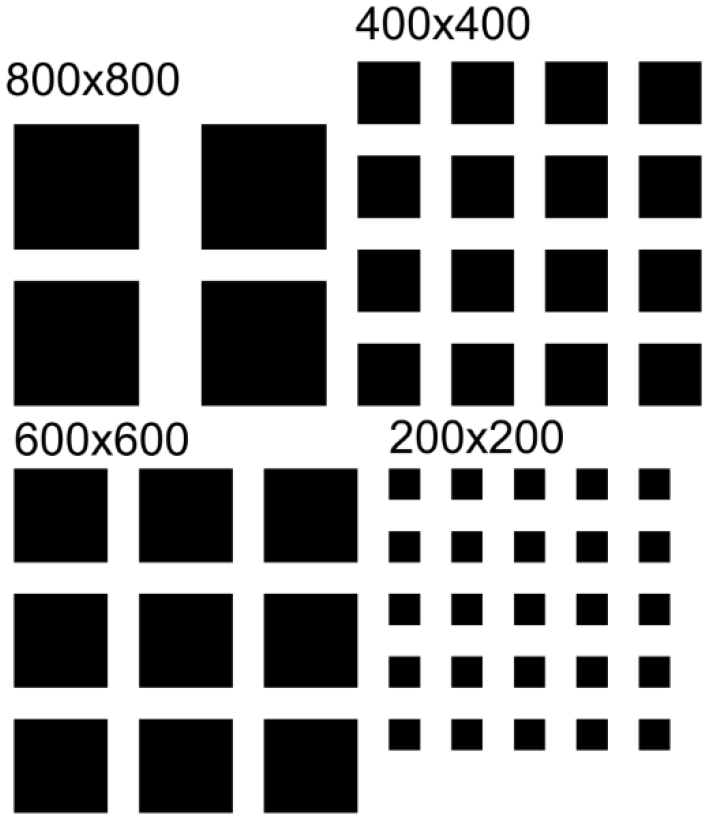
\includegraphics[width=0.8\textwidth]{Chapter3/Figs/a.png}
    \caption[Device Structure]{Photolithographic mask (left) and dimensions of the top electrical contact (right).}
    \label{fig:3a}
\end{figure}

\noindent To increase adhesion, a second titanium buffer layer is placed between the top metal contact and the oxide. This adhesive layer is less than ideal since it can cause additional imperfections to migrate within the oxide. Despite this worry, research using electron energy loss spectroscopy (EELS) and transmission electron microscopy (TEM) have shown no evidence of titanium interface migration in the devices \cite{mehonic2017intrinsic}. \\

\noindent The utilisation of gold as a primary electrical contact may result in the migration of gold atoms into the oxide layer and their subsequent diffusion through the film. For instance, a study conducted into the diffusion of gold through amorphous SiOx observed the migration of gold into the oxide when the gold was held at a temperature of $390^{\circ} C$ for a period of four hours \cite{madams1974migration}. \\

\noindent Furthermore, it was established that when the gold was exposed to a temperature of $500^{\circ} C$ for a duration of two hours, it was observed to be distributed uniformly throughout the oxide layer, which had a thickness of approximately 500 nm. Nonetheless, no migration was observed at temperatures below $370^{\circ} C$. Although the diffusion of gold through silicon oxide films at elevated temperatures has been observed, this phenomenon is frequently disregarded or presumed to be non-occurring in devices utilised as resistance switching memories. \\

\noindent In the domain of electrochemical metallisation, where metallic filaments are formed between two electrodes, gold is recognised as an inert electrode \cite{kozicki2016electrochemical}. This principle is also widely accepted in the context of valence change memories \cite{ge2014electrode}. In one particular instance of a device composed of gold and silver electrodes that were sandwiched between an $As_2S_3$ film, only the migration of silver was observed. \\

\noindent This migration resulted in the formation of a conductive bridge between the contacts \cite{hirose1976polarity}. The stability of the gold contacts within this application is assumed to be due to the fact that device operation is restricted to room temperature experiments. Alternatively, the presence and migration of a comparatively more active/mobile electrode, such as silver, may have a more significant effect on device properties.\\

\noindent It has been claimed that asymmetry in the device's construction, as well as an active and inert electrode, are necessary to identify stable switching. The molybdenum contact can be crucial as an oxygen reservoir, rapidly exchanging oxygen between the electrode and silicon oxide layer, which is similar to an active electrode, according to a recent experiment \cite{cox2021nanoscale}. The materials used for the top and bottom electrodes are different and weren't explicitly chosen for this project; rather, other group members had already picked them to create high-performance resistance switching memory. \\

\noindent The device layers remain mostly unchanged throughout the investigation. The top electrical contact is made of a different material in the experiment than the bottom electrical contact, which is made of a thin film of molybdenum. The oxide layer is made of an amorphous silicon oxide thin film. The selection of gold as the top electrical contact may cause gold atoms to diffuse through the film and migrate into the oxide. \\

\noindent Although gold has been seen to diffuse through silicon oxide layers at high temperatures, resistance switching memory frequently overlook this phenomenon or presume it does not happen. A profilometer is used to assess the thickness of the layers. To guarantee excellent conductivity throughout the device, the bottom electrode is 300 nm thick. The oxide slim film is 35nm in depth. The thickness of the top electrical contact varies depending on the substance; gold has a thickness of 110 nm, while ITO has a thickness of 50 nm.

\subsection[Manufacturing Steps]{Manufacturing Steps}

\noindent RF sputtering, a physical vapour deposition process, was used to deposit all of the device layers. Deposition is carried out at low pressure in a typical inert gas environment by blasting the intended material with a plasma, which causes the expulsion of atoms from the target. Depending on the gas pressure inside the chamber, the expelled atoms either follow a direct ballistic path or take a random walk until they land on the sample. A greater gas pressure will result in more collisions and an increased random walk, whereas a lower gas pressure produces a more direct ballistic trajectory. \\

\begin{figure}[htbp!] 
    \centering    
    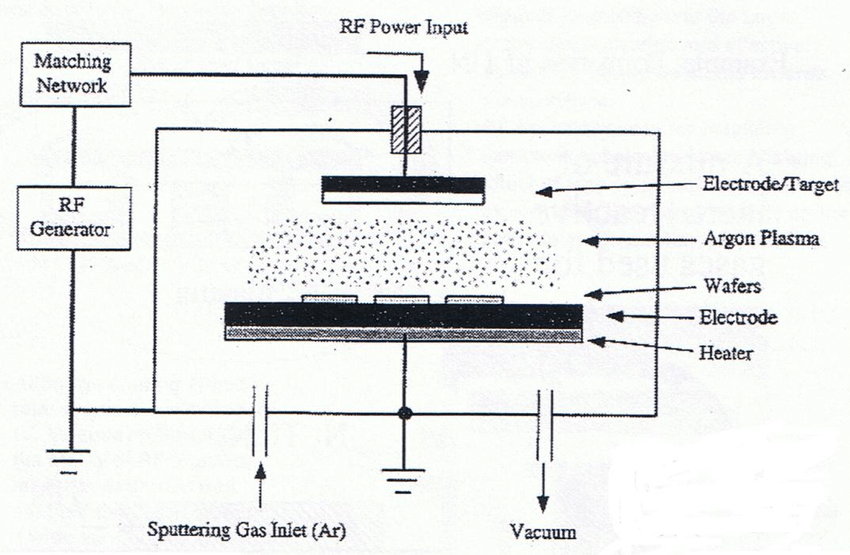
\includegraphics[width=0.6\textwidth]{Chapter3/Figs/b.png}
    \caption[Radio Frequency Magnetron Sputtering]{Depiction of the fundamental configuration for the deposition of thin films by means of sputtering \cite{jeong2008origin}. A substantial radio frequency electric field is required to ionise argon gas, thereby producing a plasma. The process of deposition is initiated by high-energy collisions between the ionised argon and the target material. The collisions result in target atoms being ejected from the source with high kinetic energy. These atoms traverse the chamber and deposit onto the sample over time, thereby forming an amorphous thin film.}
    \label{fig:3b}
\end{figure}

\noindent A simplified version of the sputtering system is illustrated in Figure \ref{fig:3b}. The configuration under consideration comprises the sample, which is connected to the anode of the RF power source, the target material, which is situated in front of the cathode, and the sputtering gas, which is injected into the chamber. The plasma is composed of argon ions, which possess a positive charge. These ions are attracted to the cathode, which is negatively charged and is therefore known as the target. The process of high-energy collisions between argon ions and the target surface is a prerequisite for the ejection of target atoms.\\

\noindent  The substance being deposited, known as the target material, is initially solid. By applying a strong electric field to the sputtering gas (argon), the plasma is created. Either a DC or an AC field is possible. However, an AC field that oscillates at an RF frequency of 13.56MHz is necessary for dielectric targets like $SiO_2$. Sputtering often results in amorphous films with sub-stoichiometric oxides. The devices' SiOx oxide has a stoichiometry of 1.9, while the film's roughness appears to be determined by the RMS roughness of the underlying molybdenum layer, which ranges from 0.9 to 1.5 nm \cite{kenyon2019interplay}. \\


\begin{figure}[htbp!] 
    \centering    
    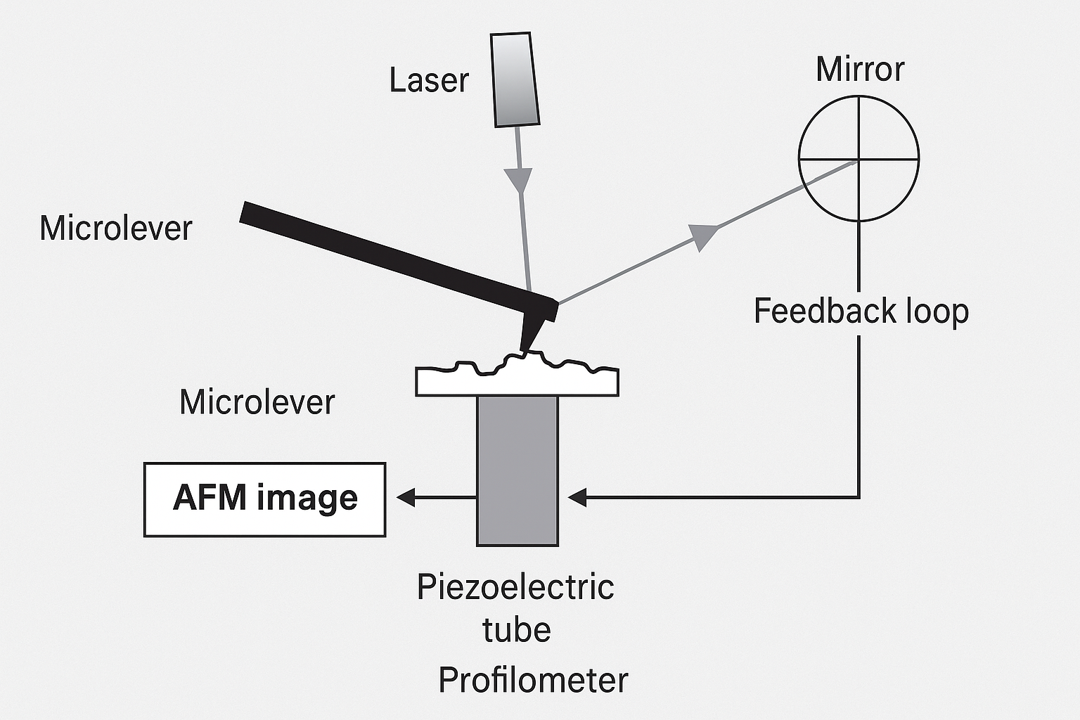
\includegraphics[width=0.6\textwidth]{Chapter3/Figs/c.png}
    \caption[Contact profilometer for thin film thickness measurements.]{Schematic of a profilometer \cite{mabilleau2008vitro}. The probe is utilised to scan the surface of the sample, with the height of the probe being adjusted accordingly in order to ensure that a constant force is maintained. It is imperative to note that a feedback loop is utilised in order to ensure the maintenance of this force during the process of reporting the tip height. The measurement of thin film thicknesses following deposition is achieved through the fabrication of a staircase-like structure.}
    \label{fig:3c}
\end{figure}

\noindent In the course of each SiOx sputtering run, a pair of Si substrate specimens are inserted into the chamber in conjunction with the sample for the purpose of thickness measurement. In the first instance, a specific region of the Si substrate is masked using a patterned photoresist. Following the process of SiOx deposition, the mask material is removed using a solvent, thereby creating a step on the SiOx/Si interface. \\

\noindent The measurement of this step is then undertaken with the aid of a Dektak XT profilometer, which is capable of resolving a step height of a few nanometres. The second piece of Si substrate, which has been covered with SiOx, is then measured using ellipsometry. This is a process that is used to verify the thickness of the deposited layer.\\

\noindent After being sputtered, film thickness is measured via a contact profilometer with a 0.5nm precision. During this procedure, a diamond tip is used to make contact with the sample and scan across the surface. Utilising a feedback loop, the tip's height is adjusted to maintain a consistent force against the sample's surface as it scans, giving the measurement of the sample height. The sample's surface height changes in direct proportion to the change in tip height. Layer thicknesses of a device stack are measured in relation to one another using a staircase-like pattern that is created during production. 

\subsection[Experimental Setup]{Experimental Setup}

The amount of current passing through the device is the significant observable. This includes details on the oxide layer's bulk conductivity as well as the interface barrier heights. The difficulty, however, is in minimising any deviations or nonlinearities brought on by the measuring apparatus itself, with probe contact resistance serving as one such example. It is necessary to choose how to make contact with the device electrodes before conducting current measurements. There are essentially two methods: either the circuit is wire bonded inside a chip carrier, or the contacts are directly probed with tiny metallic probes using micromanipulators. \\

\noindent The direct probing method utilising tungsten probes has been adopted instead due to the devices' design and susceptibility to break from the wire bonding procedure. The tip of the probe must be brought down carefully to prevent damage. When placing the probe into contact, a low voltage is often supplied as a test signal. \\

\noindent To determine if the probe has made contact, the current is watched for a spike in the device current. Initially, because there is no measurable electrical current while the probe is not in touch with the device, the current oscillates around positive and negative currents at 0 amps. Once the probe makes contact with the device, the voltage that has been applied across it now causes a detectable current that matches the polarity of the applied voltage. \\

\noindent In contrast to the probe method, which can be vulnerable to sample damage brought on by the experimentalist, the wire-bonded approach has the advantage which the position of the electrical connection does not change between experiments, thermal expansion while temperature measurements will not significantly affect the contact, and there is less risk of deteriorating the device throughout characterisation. \\

\noindent However, there is a chance that the component will be broken during the bonding procedure with wires. An ultrasonic pulse is utilised to melt a gold or aluminium wire to the device contact while applying pressure to help fuse the two metals together. It has been regularly observed that this pressure can cause internal layers to compress, leading to electric shorts between the two metal contacts and ultimately damaging the device. \\ 

\begin{figure}[htbp!] 
    \centering    
    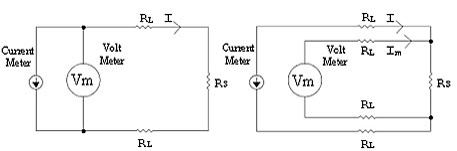
\includegraphics[width=0.8\textwidth]{Chapter3/Figs/d.png}
    \caption[Two wire or Four wire (Kelvin) testing.]{Two wire or Four wire (Kelvin) testing. A schematic of the 2-wire measurement setup is provided herewith. The voltage (VSource) is applied to the sample using two probes. It is important to note that each probe introduces a series resistance (Rprobe) with the sample's resistance (Rsample). The device current (Imeas) is measured by an ammeter in series. Conversely, a constant current (Isource) is supplied through the sample by two probes. The voltage induced across the device (Vmeas) by the current is measured with a voltmeter in parallel with the sample.}
    \label{fig:3d}
\end{figure}

\noindent After deciding on a contact technique, the next choice is how currents will be monitored. Both a 2-wire measurement and a 4-wire measurement are frequently available as options. The sample's conductivity serves as the basis for the decision. The easiest way to measure electrical resistance is to apply a set voltage and track the total current passing through the object. Only two electrical connections are formed, thus the term "2-wire measurement" for this procedure. Ohm's Law is used to determine the device resistance by connecting a voltage source, an ammeter, and the device in series. \\

\noindent Due to the assumption that the electrical resistance is only determined by the test device, which is not true in reality where there are several sources of electrical resistance connected in series with the device, this measurement is often not correct. These include the wires connecting the test object and the voltage source, the internal resistance of the voltage source or the ammeter, and, especially, the contact resistance that develops at the point where the electrical probes and the test object meet. \\

\noindent One of the most crucial parameters to take into account when describing thin films is contact resistance, which may be reduced by placing metal contacts on the sample during manufacturing. Fortunately, the device resistance usually outweighs the electrical resistance, making this method valid in the majority of instances. However, when resistance is small, the parasitic resistances of the measuring circuit become notable and must be eliminated by using a 4-wire resistance measurement. \\

\noindent Ohm's law is still used in this configuration to calculate resistance. Instead of sourcing a voltage and monitoring a current, the device is subjected to a steady current that induces a voltage across it. Through two extra probes connected in parallel to the device, a voltmeter measures the potential decrease. It is crucial to recognise that the same contact resistance and wire resistances that plagued the 2-wire method continue to exist for all four connections. However, in this case, the high impedance of the voltmeter causes a substantially lesser current to pass through the measuring contacts. \\

\noindent The voltage recorded by the voltmeter is thought to more precisely represent the voltage drop across the device since the voltage dip across the parasitic resistance is insignificant. This occurs because the voltage produced across the contact resistance is lowered as a result of the reduced current flowing through the probes, which detect the voltage across the device. By lowering these voltages, which are induced across each probe's contact resistances and contribute mistakes into the voltage measurements, it is possible to measure the voltage across the device with more accuracy. \\

\noindent Thus, the device resistance determines whether to use a 2-wire or 4-wire resistance measurement. The devices examined in this work have high resistance, ranging from kilo-ohms to mega-ohms. The parasitic resistances of the measuring circuit, like the contact resistances, are insignificant at this level. The issue of measuring device currents must now be solved once the device has been attached. Again, there are a variety of techniques that might be applied; the one selected will often depend on the size of the current being measured. \\

\noindent The most elementary method of measuring current is to use a digital multimeter (DMM) ammeter. The device functions in accordance with Ohm's law, utilising the principle of electrical resistance to measure the voltage drop across a fixed resistor, commonly referred to as the shunt resistor. Whilst the validity of this approach is indisputable for currents within the milliamp range and above, issues arise for lower current levels due to the noise induced by the shunt resistor.  In order to measure smaller currents, larger shunt resistors are required. This, however, gives rise to two problems. \\

\noindent Firstly, it is important to note that larger resistors are known to introduce greater thermal noise, which has the capacity to disturb the voltage being measured. Secondly, an increase in resistance results in an increase in the voltage drop across the ammeter. The voltage drop, termed the 'voltage burden', becomes problematic when its magnitude is no longer negligible in comparison to the voltage applied to the device under test. The combination of voltage burden and the thermal noise of the shunt resistor invariably imposes a lower limit on current measurements when a DMM is employed. \\

\noindent The average current range for the devices is 100nA to 1mA, therefore a picoammeter is required to detect considerably lower currents on the order of picoamps to nanoamps. Picoammeters minimise current readings by a number of methods that differ across manufacturers. The majority of them employ a transimpedance amplifier to magnify the signal while an op-amp converts the input current to a voltage. Once again, how this is implemented differs from manufacture to manufacture and is frequently protected intellectual property that is not revealed. \\

\begin{figure}[htbp!] 
    \centering    
    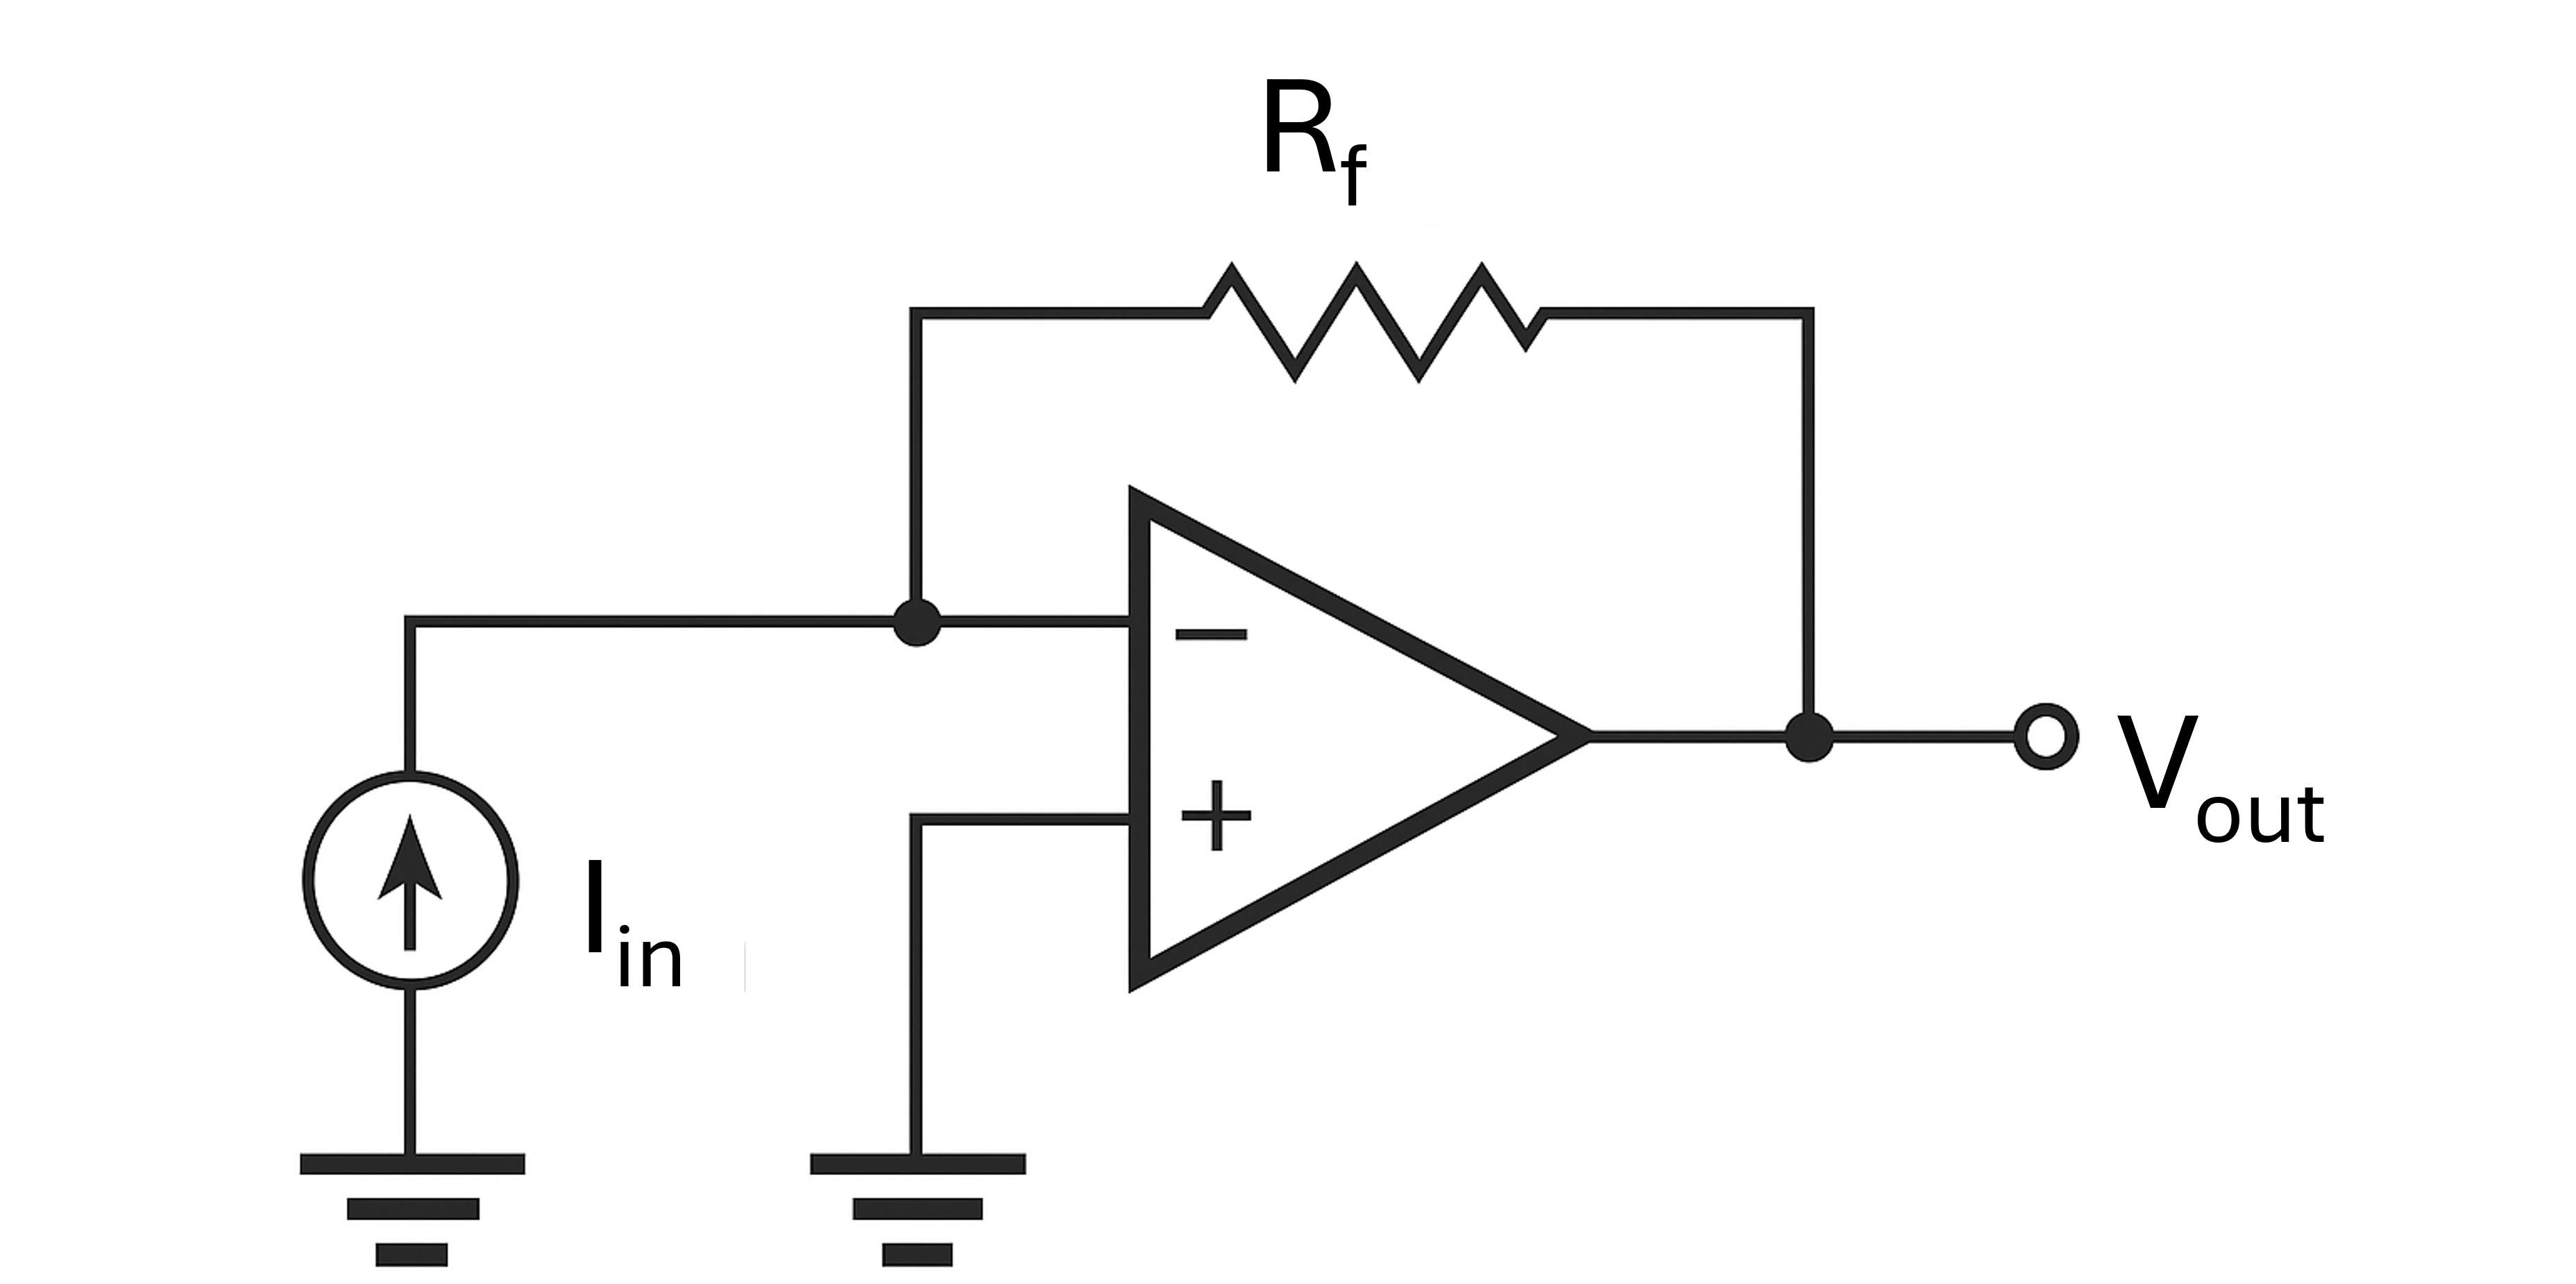
\includegraphics[width=0.5\textwidth]{Chapter3/Figs/e.png}
    \caption[Transimpedance amplifier circuit.]{Transimpedance amplifier circuit. The input current ($I_{in}$) is amplified and converted into an output voltage ($V_{out}$) via the operational amplifier. The gain is defined by the feedback resistor (RF). The voltage/current ($V_{out}/I_{in}$) is equivalent to negative resistance ($-R_f = V_{out} / I_{in}$).}
    \label{fig:3e}
\end{figure}

\noindent Nevertheless, the general operation can be comprehended with the aid of the circuit in Figure 8. The circuit under consideration is a transimpedance amplifier, the function of which is to convert the input current ($I_(in)$) to an output voltage ($V_(out)$). The operational amplifier is known to adjust its output voltage in order to reduce the voltage difference between its two input pins, designated as '-' and '+'. In this circuit, the non-inverting input pin (+) is grounded. This action causes the operational amplifier (op-amp) to adjust its output voltage, thereby ensuring that the voltage at the inverting input pin (-) is also zero volts. \\

\noindent The application of an input current to the circuit results in a transient voltage offset at the input pin. The op-amp rapidly adjusts the output voltage, thereby inducing a current of equal and opposite magnitude through the feedback resistor. This, in turn, results in the cancellation of the input current. The voltage at the inverting pin (-) is rapidly returned to zero by the feedback from the operational amplifier, thereby creating a virtual ground. \\

\noindent The generation of this inverse current ($I_{inv}$) is accompanied by the definition of the voltage at the output of the operational amplifier in accordance with Ohm's law: It can thus be demonstrated that the voltage is $V_{out} = -R_f \cdot I_{inv}$, resulting in a voltage that follows the input current. The amplification of this voltage is defined by the feedback resistor, $R_f$. The virtual ground is a key advantage of this technique. The consequence of this is a significant reduction in the voltage burden, since the shunt resistor that was previously connected in series with the device under test has now been removed. This facilitates the measurement of smaller currents, which would not have been possible using a DMM due to the significant voltage burden caused by the sensing resistor. \\

\noindent It is evident that, in view of the aforementioned factors, the utilisation of a picoammeter constitutes the optimal instrument for the execution of current-time measurements or current-voltage sweeps on our devices The equipment used in this instance is the Keithley 6430 sourcemeter, which combines a picoammeter and a low noise voltage source into a single device. \\

\begin{figure}[htbp!] 
    \centering    
    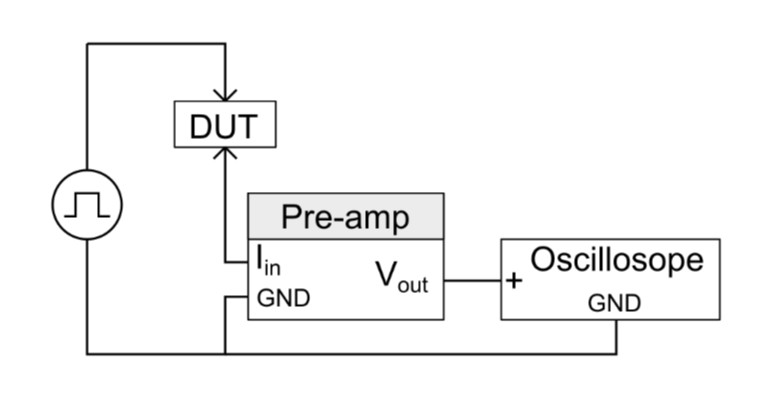
\includegraphics[width=0.8\textwidth]{Chapter3/Figs/f.png}
    \caption[Experimental setup of spike train measurements.]{Experimental setup of spike train measurements. Spike trains are generated using an arbitrary signal generator. The device current is amplified and converted into an output voltage via the preamplifier, which is connected in series with the device. The output of the current preamplifier is then captured by an oscilloscope.}
    \label{fig:3f}
\end{figure}

\noindent In some cases, the device requires the application of voltage transients that are more complex than step potentials, such as pulses or custom spike trains. In these cases, the Keithley's sampling frequency is insufficient to generate such signals. An arbitrary signal generator is used in its place to create voltage transients, and a current preamplifier is connected in series with the device to amplify device currents. In particular, the oscilloscope (Rigol DS4024) and current preamplifier (SR570) are used.

\section[Electrical Characterisation]{Electrical Characterisation}

\noindent Resistive switching is defined as a reversible phenomenon that occurs in two-terminal elements. In a non-volatile manner, these devices undergo a change in resistance when subjected to electrical stimuli. In the case of ReRAM devices, it is a local redox process that dictates the resistive switching mechanism. The reversibility of the process is achieved by the repeated application of suitable stimuli. This mechanism governs the resistance values between two or more levels. \\

\noindent The predominant phenomenon observed in these devices is resistive switching. For the sake of convenience, the switching states of the memristor can be defined. The assignment of high resistance to the "OFF" state and low resistance to the "ON" state is intuitive, with a contrast in resistance by a few orders of magnitude. The transition from the high resistance state (HRS) to the low resistance state (LRS) is defined as "Set", while the reverse is defined as "Reset". In many cases, an initial electroforming process is required to transform the device from a pristine state to a switchable state. It is generally accepted that the pristine device exhibits a higher degree of resistance than the HRS.\\

\noindent The majority of metal oxide devices exhibit either unipolar or bipolar switching. In contrast, both unipolar and bipolar switching can be observed in our silicon oxides. The preliminary characterisation of these devices encompassed the fundamental I-V characteristics. The experimental procedure involved the execution of the tests utilising the dual sweep functionality of the Keithley 4200-SCS, employing two tip probes with a diameter of 10 $\mu m$. Testing was performed on both sets of samples across all electrode pad sizes.

\subsection[Unipolar Switching Mode]{Unipolar Switching Mode}

\noindent Initial electroforming is a prerequisite for switching in these devices. It is generally accepted that fresh samples are in a very HRS, which necessitates the application of a significant electrical stimulus to enable the cell to transition into LRS for the first time. Subsequent to this preliminary phase of formation conditioning, the apparatus may be reversibly switched between two bi-stable states. \\

\begin{figure}[htbp!] 
    \centering    
    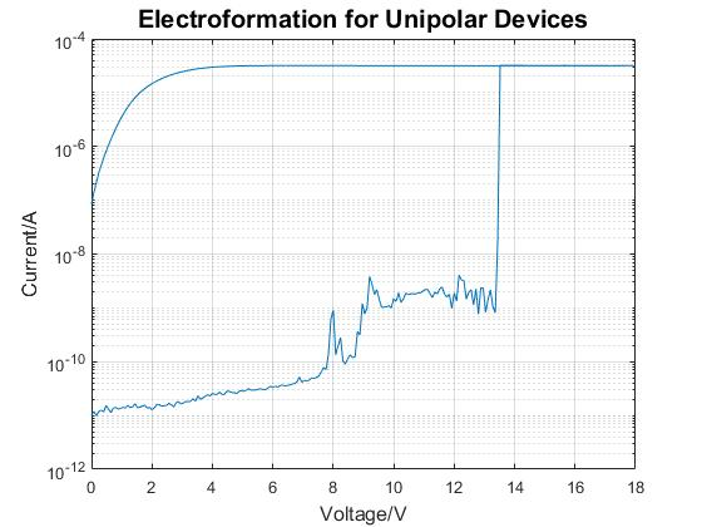
\includegraphics[width=0.7\textwidth]{Chapter3/Figs/g.png}
    \caption[Initial Electroformation step for unipolar switching.]{Initial Electroformation step for unipolar switching via a double sweep curve.}
    \label{fig:3g}
\end{figure}

\noindent The electroforming operation is widely regarded as a form of electrical breakdown, which is critically dependent on current-limiting mechanisms to ensure the subsequent switching functionality of the cell. Current limitations may be addressed by leveraging the existing compliance functionality of the Keithley-SCS. In certain instances, the analyser may exhibit a slower response rate than the formation process itself, resulting in overshoot phenomena during practical applications. It is imperative to note that this electroformation step is only performed once to pristine devices. \\

\noindent The operation is conducted through the programming of the Keithley-SCS to sweep at an elevated voltage of up to 18V, as illustrated in Figure \ref{fig:3g}. During the process of sweeping, it is possible to observe a number of current peaks with the I-V curve displaying an unstable state. Once a sufficiently high voltage is reached, approximately 14V in this case, the device abruptly switches into LRS. Subsequent sweeps are found to be of a more even and refined nature when compared with the preceding sweep. \\

\begin{figure}[htbp!] 
    \centering    
    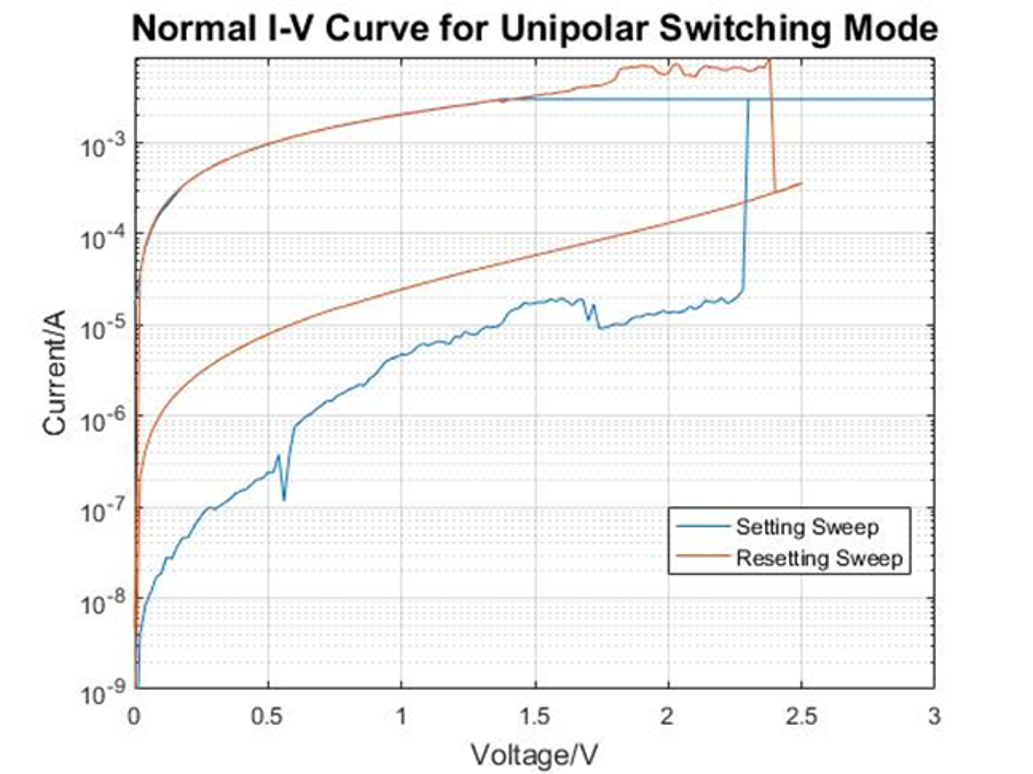
\includegraphics[width=0.7\textwidth]{Chapter3/Figs/h.png}
    \caption[Non-volatile switching behaviour for unipolar device under current compliance.]{Non-volatile switching behaviour for unipolar device under current compliance.}
    \label{fig:3h}
\end{figure}

\noindent The observed change in conductance may be attributed to structural changes occurring during the forming process, possibly resulting from a reduction step that involves the removal of oxygen from silicon oxide, thereby forming oxygen vacancies. Following the electroformation step, the LRS demonstrates stability. The device maintains its state subsequent to the removal of the electrical stimulus, thereby exhibiting non-volatile switching characteristics. It is important to note that the initial very HRS is never recovered. \\

\noindent As demonstrated in Figure \ref{fig:3h}, the unipolar switching mechanism is evident in the initial set of symmetrical MIM devices. The blue plot indicates the Set process, whereby the device transitions from the "Off" state to the "On" state at a specific threshold voltage, approximately 2.3V in this instance. \\

\noindent In this instance, the sweeping voltage has been configured to 3V with 3 mA current compliance, a setting sufficient for the switching process to occur. It has been demonstrated that a reduction in voltage below the threshold does not result in the device transitioning to its previous state.\\

\noindent It is evident that a critical current must be attained for the purpose of resetting the device. The Reset process can be observed in the orange plot, which displays a larger current, approximately one order of magnitude greater than the setting current compliance. This results in the device being restored to HRS. \\

\noindent The phenomenon of Joule heating is induced by high-current flow, resulting in localised heating and device reset. In the absence of current compliance, the device may undergo a hard breakdown or exhibit multiple transitions between the two states. It is important to note that the switching sequence can be performed repeatedly.\\ 

\begin{figure}[htbp!] 
    \centering    
    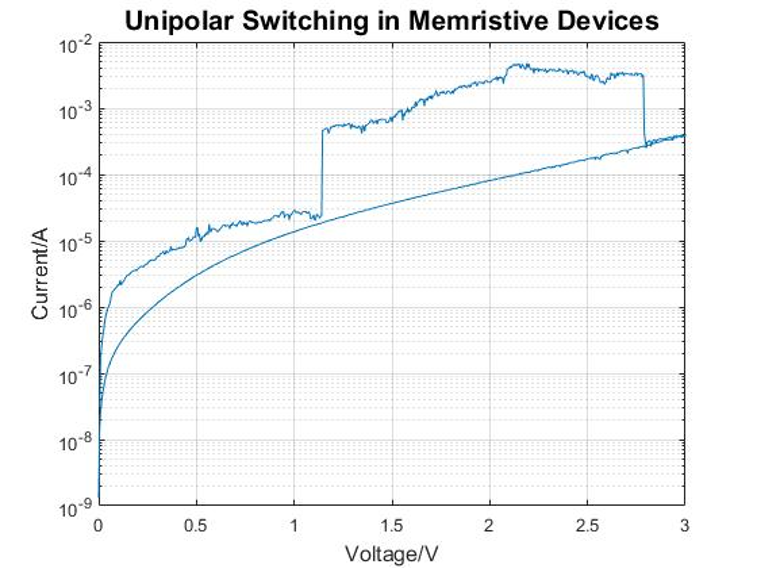
\includegraphics[width=0.7\textwidth]{Chapter3/Figs/i.png}
    \caption[Observation of Set and Reset process under the same sweep.]{Observation of Set and Reset process under the same sweep.}
    \label{fig:3i}
\end{figure}

\noindent The HRS conductance remains in a state between that of the LRS and the pristine state. In both cases, the transition is found to be abrupt and independent of the sweeping parameters, in contrast to the ideal pinched hysteresis loop suggested in the previous chapter. In summary, an elevated magnetic field is likely to set the device in the LRS, whereas high Joule heating is likely to reset the device to the HRS.\\


\noindent An alternative mechanism for unipolar switching can be observed in Figure \ref{fig:3i}. Devices with a setting voltage lower than the reset voltage will transition to LRS at a lower voltage. Subsequently, these devices will return to HRS at a higher voltage, which in this case is 1.15V and 2.85V, respectively. There is no current compliance requirement for this type of unipolar switching with reset occurring when the current has reached a critical value. \\

\begin{figure}[htbp!] 
    \centering    
    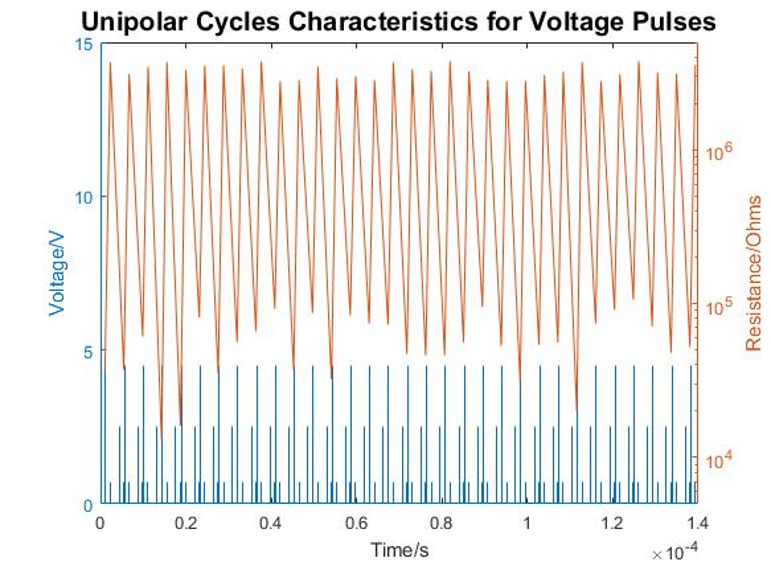
\includegraphics[width=0.7\textwidth]{Chapter3/Figs/j.png}
    \caption[Observation of Set and Reset process under the same sweep.]{Observation of Set and Reset process under the same sweep.}
    \label{fig:3j}
\end{figure}

\noindent As illustrated in Figure \ref{fig:3j}, the unipolar device undergoes cycling under conditions of stress testing. The blue spikes in the diagram represent voltage pulses that are utilised to switch the devices in positive bias. The device is set using a short voltage pulse of 4.5 V, with a duration of 100 ns. In order to effect a reset of the device, a longer voltage pulse of 2.5 volts at 2 milliseconds was utilised in order to accommodate Joule heating. \\

\noindent It was observed that each setting and resetting pulse was succeeded by a subsequent reading pulse of 0.7 V at 1 ms. The amplitude of this reading pulse is sufficiently small to avoid interfering with the set and reset process, while providing a clear reading that can be seen in the orange plot. It is evident that under typical operating conditions, the cycling resistance readings exhibit a discrepancy that is at least two orders of magnitude apart.\\

\begin{figure}[htbp!] 
    \centering    
    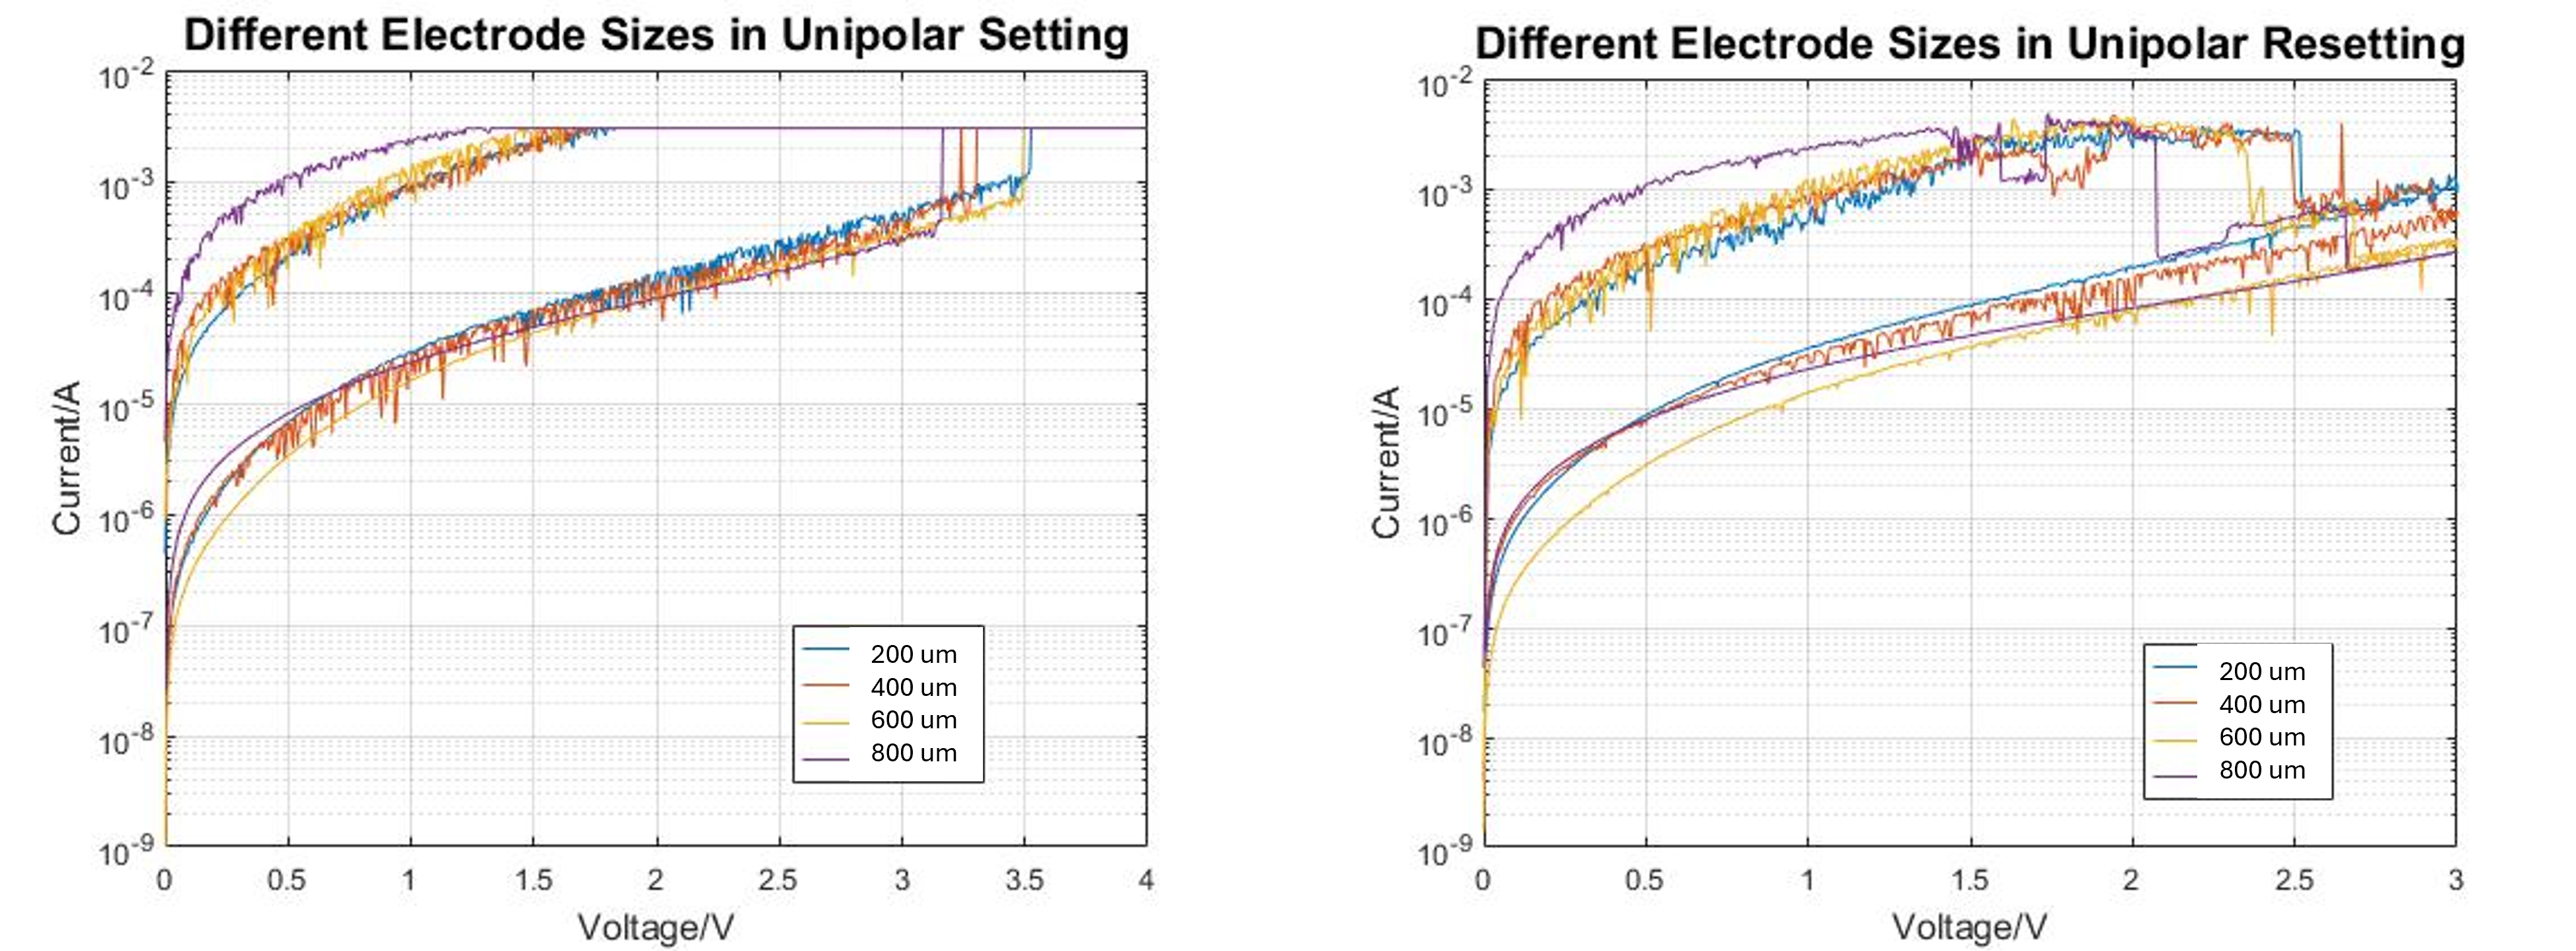
\includegraphics[width=1\textwidth]{Chapter3/Figs/k.png}
    \caption[Switching in unipolar devices across different electrode sizes.]{Switching in unipolar devices across different electrode sizes.}
    \label{fig:3k}
\end{figure}

\noindent It was also demonstrated that switching in unipolar devices is independent of electrode size. Figure \ref{fig:3k} shows that the switching processes for square contacts ranging from 200 x 200 $\mu m$ to 800 x 800 $\mu m$ are comparable. The devices consistently switch at around 3.5 V and 3 mA of current compliance. Similarly, the reset process is consistent when the samples reach the critical current threshold of approximately 5 mA.

\subsection[Bipolar Switching Mode]{Bipolar Switching Mode}

\noindent  Bipolar switching results were obtained from a set of asymmetric devices with Mo/SiOx/TiAu construct. As with unipolar devices, asymmetric bipolar devices require an initial electroforming step before the samples can be cycled between two distinct states. Figure \ref{fig:3l} shows the electroforming process in bipolar devices. A dual voltage sweep is applied to the sample up to -10 V at a current compliance of 0.1 mA. As with the unipolar devices, the sample exhibits some unstable spiking activity as the voltage sweeps from a pristine HRS to a LRS.\\


\begin{figure}[htbp!] 
    \centering    
    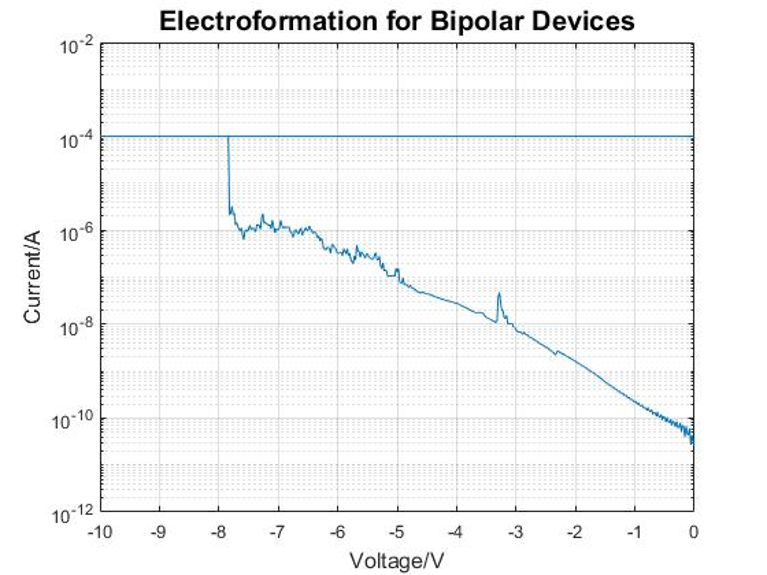
\includegraphics[width=0.7\textwidth]{Chapter3/Figs/l.png}
    \caption[Initial electroformation step for unipolar sample via a double sweep curve.]{Initial electroformation step for unipolar sample via a double sweep curve.}
    \label{fig:3l}
\end{figure}


\noindent Following the conclusion of the preliminary electroforming process, the apparatus is capable of reliably transitioning between two stable states. As illustrated in Figure \ref{fig:3m}, the device transitions between two distinct resistance states through the application of voltage stimuli of opposite polarity. The device is set using a negative voltage sweep up to -2V. \\

\begin{figure}[htbp!] 
    \centering    
    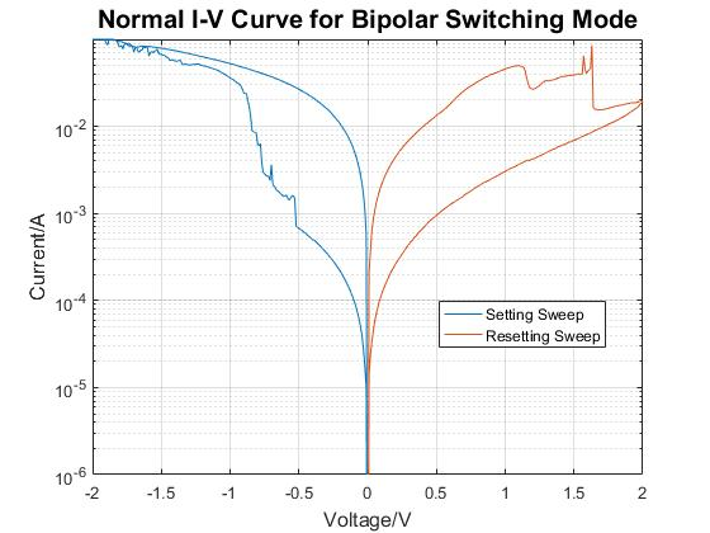
\includegraphics[width=0.7\textwidth]{Chapter3/Figs/m.png}
    \caption[Observation of bipolar switching in asymmetric device with -2V Set and 2V Reset sweeps.]{Observation of bipolar switching in asymmetric device with -2V Set and 2V Reset sweeps.}
    \label{fig:3m}
\end{figure}

\noindent The current compliance was set at 100mA in order to demonstrate a clear transition between the two states, with the conductance changing by two orders of magnitude. It is important to note that a reduced current compliance should be employed in order to achieve a balance between the device's lifespan and its conductivity. The device is reset by means of an opposing 2V dual sweep of positive polarity, a process known as bipolar switching.\\


\noindent From a physical perspective, this particular type of bipolar switching mechanism is intrinsic and can be categorised as belonging to the valence change mechanism class. In this category of memory devices, the electroforming process typically leads to local reduction, thereby forming a conductive pathway. It is hypothesised that this channel is composed of oxygen vacancies, which permit oxygen ions to migrate in and out of the channel in response to an applied electric field. \\


\noindent The location of the local redox process is hypothesised to be in proximity to a filament-to-electrode interface. The effective tunnelling barrier height at this interface is indicative of the resistance state of the device. The height of this barrier is subject to variation under different applied voltage biases, thereby inducing the movement of oxygen ions and resulting in a corresponding alteration to the resistance state. \\

\begin{figure}[htbp!] 
    \centering    
    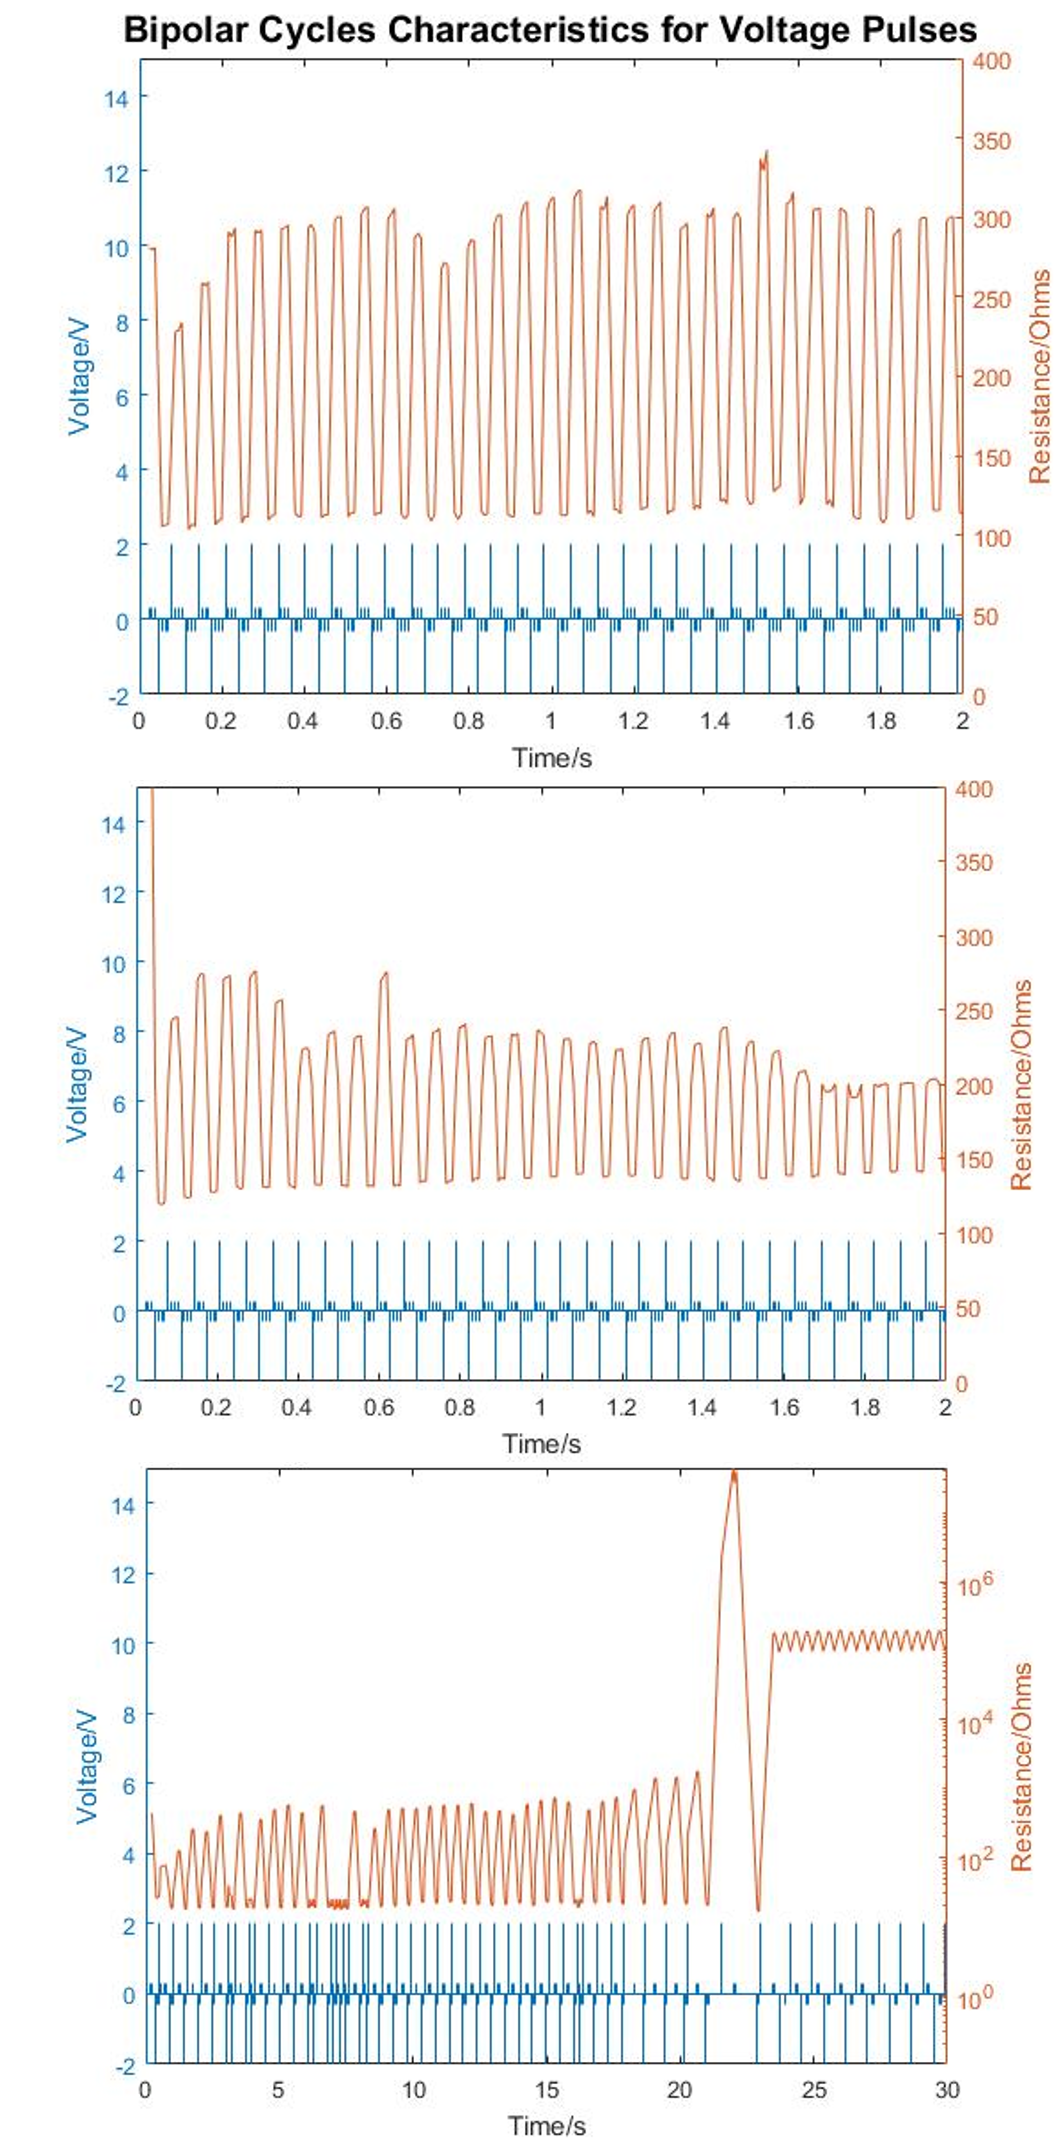
\includegraphics[width=0.65\textwidth]{Chapter3/Figs/n.png}
    \caption[Cycling stress test for bipolar devices.]{Cycling stress test for bipolar devices. Initial device cylcles (top) followed by LRS convergence (middle) and hard reset breakdown (bottom).}
    \label{fig:3n}
\end{figure}

\noindent The transition between these two resistive states can be facilitated by the application of suitable voltage pulses. As demonstrated in Figure \ref{fig:3n}, the device exhibits a high degree of reliability in its switching capability when utilising a -2 V setting, in conjunction with 2 V resetting pulses. \\


\noindent It was recorded that each setting or resetting pulse is succeeded by five 0.1V or 0.1V reading pulses for the resistive state that the device is purportedly in. In this configuration, the HRS is approximately 300$\Omega$, while the LRS is about 100 $\Omega$. It is noteworthy that the selection of these voltage pulses was made with the objective of accurately measuring the resistance, without causing the switching mechanisms of the device to be triggered.\\

\noindent In the experiment, the device demonstrated a minimum of 4500 cycles of operational longevity when subjected to a current bias of 10mA. This was followed by a convergence towards LRS, as evidenced by the switching between 200$\Omega$ and 150$\Omega$, as depicted in Figure \ref{fig:3n}. As an alternative scenario, when the device is operating at a higher current compliance of 100mA, the stress test sustains approximately 40 cycles before the device experiences irreversible failure, entering the HRS state at 200k$\Omega$. \\


\noindent Finally, Figure 35 demonstrates switching behaviours for bipolar devices across a range of contact sizes, from 200 x 200$\mu m$ to 800 x 800$\mu m$. All the setting sweeps were programmed up to -2V with 5mA current compliance for the purpose of facilitating clear transition observation. It is evident that the resetting sweep has been configured to a voltage of 2V, with a current compliance of 100mA. \\

\noindent The results obtained demonstrate some variations in the switching voltages and contrast ratio between HRS and LRS. This finding suggests the potential necessity for further statistical analysis in subsequent devices. However, it is evident that all samples demonstrate consistent switching activities within the range of voltage stimuli applied during the testing process.

\begin{figure}[htbp!] 
    \centering    
    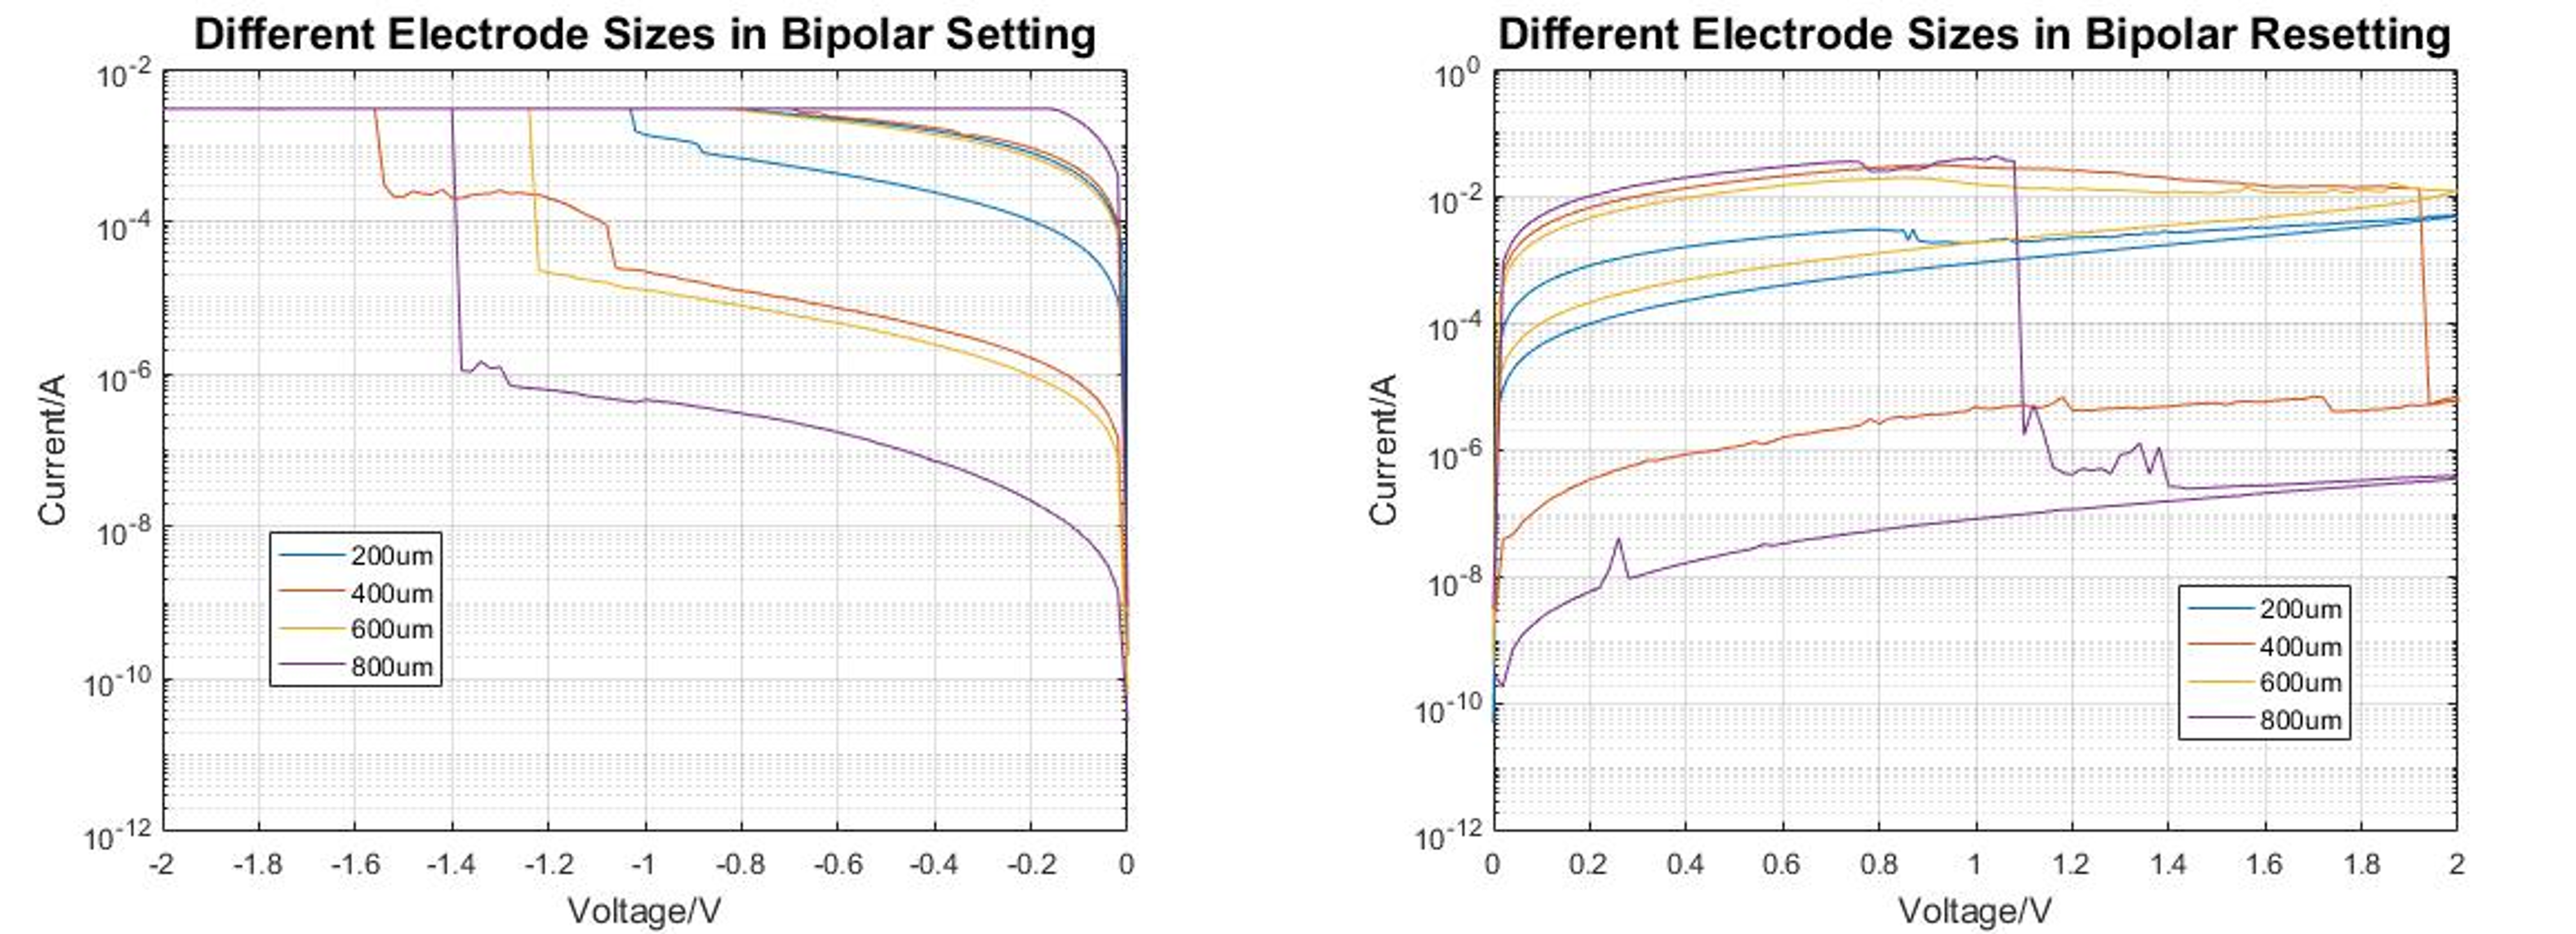
\includegraphics[width=1\textwidth]{Chapter3/Figs/o.png}
    \caption[Switching in bipolar devices across different electrode sizes.]{Switching in bipolar devices across different electrode sizes.}
    \label{fig:3o}
\end{figure}

\subsection[Alternate Operating Modes]{Alternate Operating Modes}

As demonstrated in previous observations, the switching of both unipolar and polar samples is reliable under specific, correctly configured, programming conditions. Furthermore, it appears that the switching does not scale in proportion to the electrode contact size. This finding indicates that carrier transport occurs for individual conducting filaments. However, it should be noted that certain devices exhibit alternative switching modes, namely gradual and multi-level switching modes. The presence of parallel conductive pathways within the same insulating layer is a potential cause of this phenomenon. \\

\begin{figure}[htbp!] 
    \centering    
    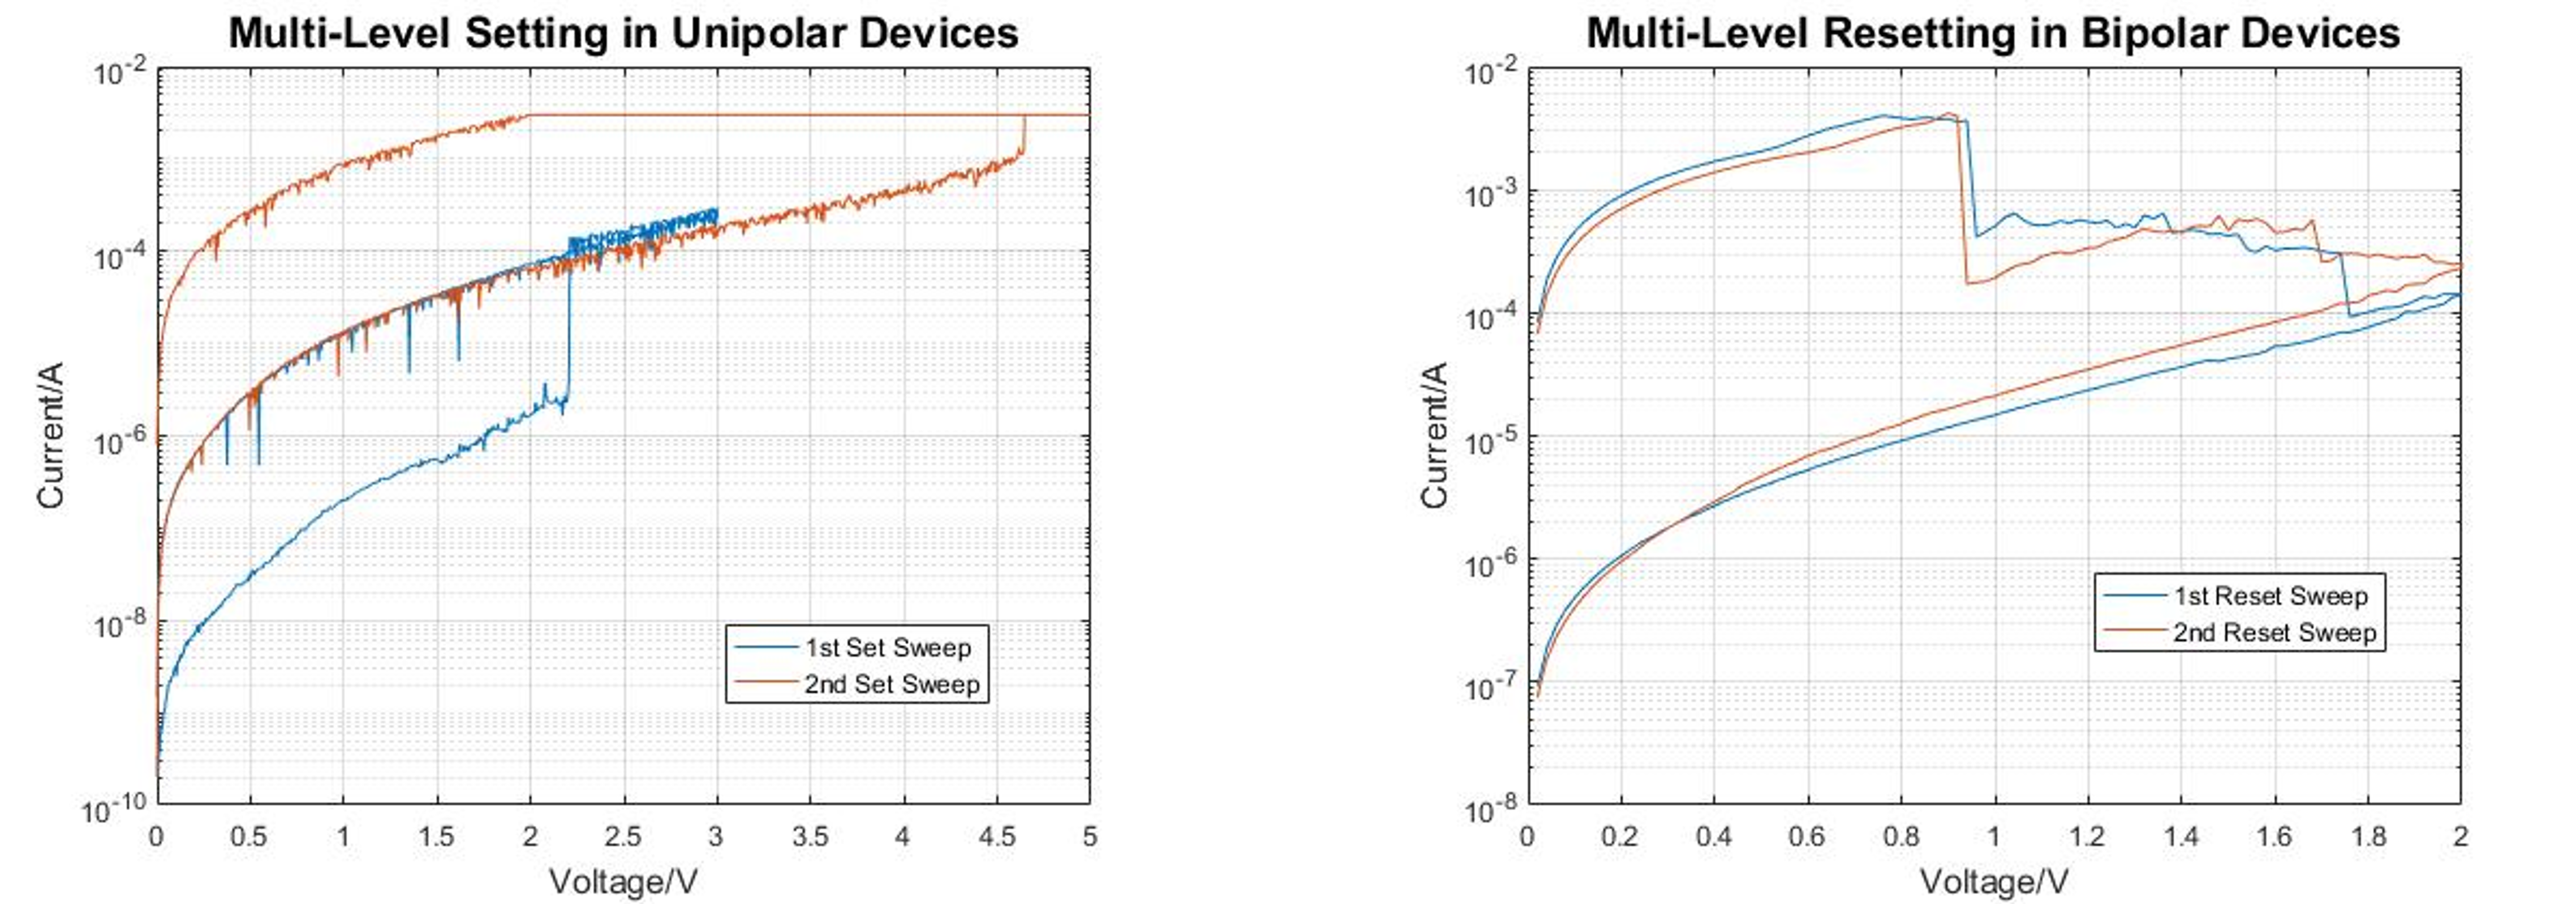
\includegraphics[width=1\textwidth]{Chapter3/Figs/p.png}
    \caption[Multi-levels I-V characteristics in MIM devices.]{Multi-levels I-V characteristics in MIM devices during the Set (left) and Reset (right) process.}
    \label{fig:3p}
\end{figure}

\noindent In both unipolar and bipolar samples, there are some devices exhibiting the multilevel switching characteristic, as illustrated in Figure \ref{fig:3p}. The initial transition process during the set stage can be followed by a subsequent stable transition to an even lower LRS, thereby providing a minimum of three or more switchable states. \\

\noindent As demonstrated above, both setting states are found to be stable, with the HRS of the second sweep coinciding with the LRS of the first sweep. The device can be configured at the first or second LRS, with two separate voltage sweep levels available for this purpose. As illustrated in the aforementioned example, the generation of the primary and secondary LRS was achieved through the utilisation of 3V and 5V sweeps, respectively.\\

\begin{figure}[htbp!] 
    \centering    
    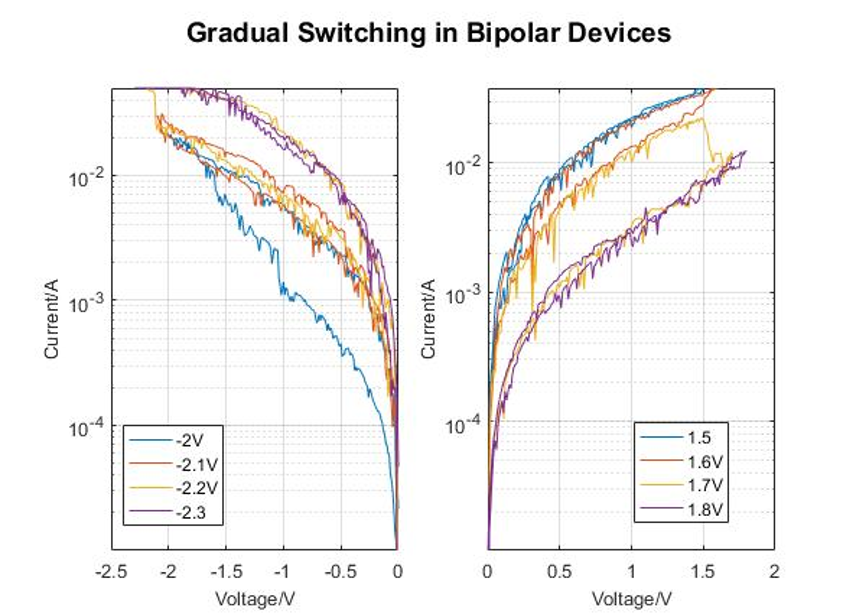
\includegraphics[width=0.7\textwidth]{Chapter3/Figs/q.png}
    \caption[Gradual increase (left) and decrease (right) in conductivity for bipolar device.]{Gradual increase (left) and decrease (right) in conductivity for bipolar device.}
    \label{fig:3q}
\end{figure}

\noindent In a similar manner, multilevel reset can be observed in bipolar samples at 1V and 1.8V, respectively. It is important to note that, in this case, the transitions window is smaller than that of the unipolar devices. In both cases, the switching is stable, with a contrast ratio between each state that is at least one order of magnitude.\\

\noindent In the case of bipolar switching samples, it is possible to observe not only the abrupt changes in resistance that are normally observed, but also gradual changes in conductivity (see Figure \ref{fig:3q}). As indicated by HRS, the gradual increase in conductance is achieved by sequentially sweeping the device with increasing setting voltage levels, ranging from -2V to -2.3V, under an appropriate stepping current compliance of 100mA in this case.\\

\noindent It has been demonstrated that a gradual decrease in conductivity is generated during the reset process, with this decrease commencing from LRS. This gradual change is obtained by progressively sweeping the device at higher potential, from 1.5V to 1.8V. The concluding phase of these procedures is characteristically sudden, thereby impeding the attainment of further transitions. The outcomes obtained were found to vary in terms of their gradualness or abruptness, suggesting the potential for further statistical analysis with reduced voltage steps in subsequent characterisations.\\

\begin{figure}[htbp!] 
    \centering    
    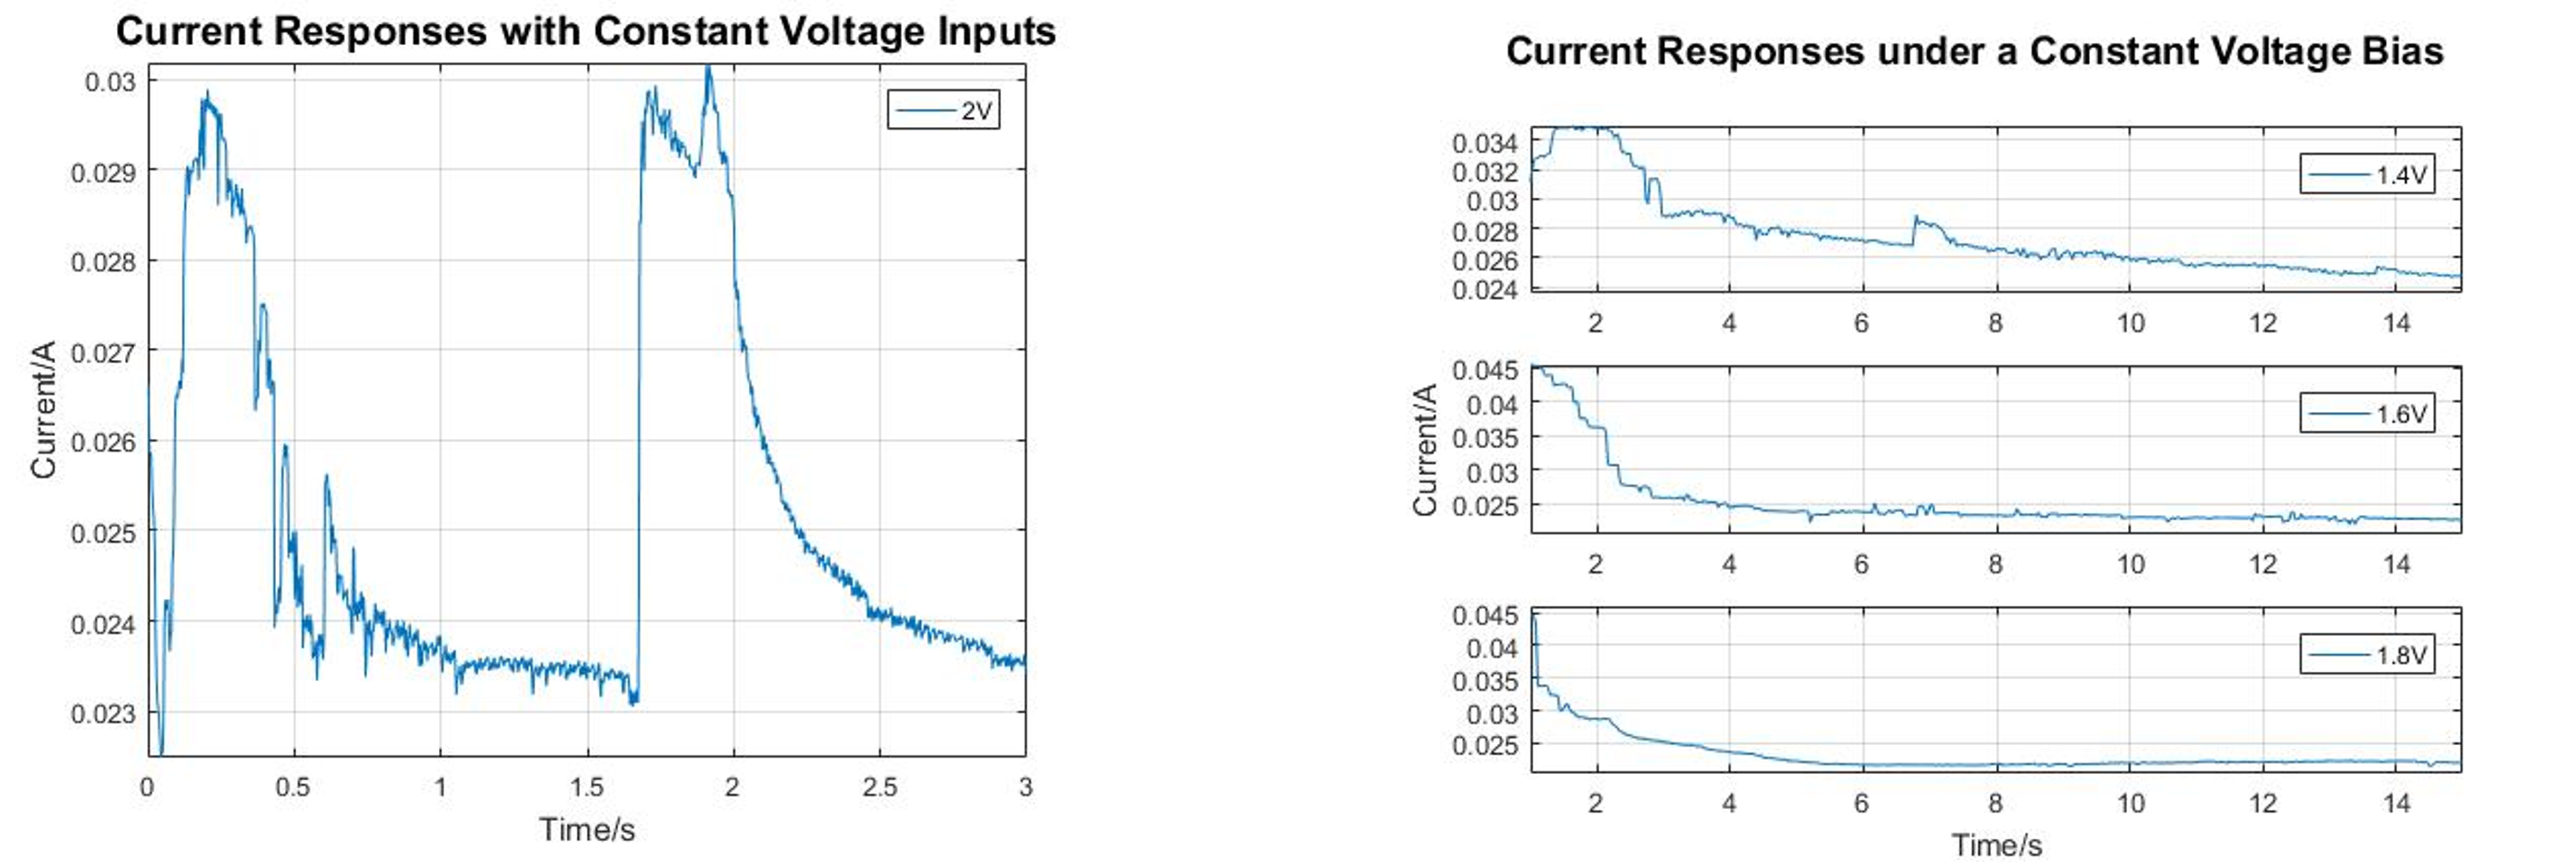
\includegraphics[width=1\textwidth]{Chapter3/Figs/r.png}
    \caption[Current-time plots showing transitions between resistive states.]{Current-time plots showing transitions between resistive states (left) and time constant comparison (right).}
    \label{fig:3r}
\end{figure}

\noindent As information processing is concerned with the manner in which data is processed over time, it is imperative to assess the performance of devices over time. In the preceding section, the switching mechanisms have been investigated with regard to time via the cycling stress tests. In this experiment, the characteristics of the device under constant voltage and current bias will be observed.\\

\noindent As illustrated in Figure \ref{fig:3r}, the current time plot for different voltage biases in unipolar samples is demonstrated. Applying a voltage of 2V to the device results in discernible transitions between the set and reset processes, with these transitions exhibiting an inverse relationship to one another. \\

\noindent It is evident that alterations in the resistive state can be observed when there is a rapid increase in the current (set), which is then shortly followed by an exponential decay (reset). The rate of recovery is indicated by the time constant of the exponential decay. A comparison of the individual inputs reveals that the time constant varies in proportion to the voltage bias. When the voltage bias increases from 1.4V to 1.8V, the time constant decreases from 7s to 1s.\\

\begin{figure}[htbp!] 
    \centering    
    \includegraphics[width=1\textwidth]{Chapter3/Figs/s.png}
    \caption[Volatile activities observed under different constant current inputs.]{Volatile activities observed under different constant current inputs for unipolar device (left) and switching at sufficiently high input current bias in bipolar device (right).}
    \label{fig:3s}
\end{figure}

\noindent When a constant current is applied to the samples, volatile spiking activities can be observed in Figure \ref{fig:3s}. It is evident that an increase in current from $5\mu A$ to $10 \mu A$, as observed for unipolar devices, results in a corresponding rise in volatility. This phenomenon can be attributed to the constant current input, which has a significant impact on the device's response. These instabilities can manifest as amplitude variations, with spikes ranging from 0.02V to 0.45V, or as timing variations, with spikes occurring more frequently at higher current biases.\\

\noindent The device exhibits spiking activities until the current bias is sufficiently large to trigger a switching transition. When the bipolar device is critically biased at -10mA, it switches shortly after exhibiting volatile activities, following an uncharacteristically large spike. Following the transition, the spiking behaviours become less predominant.

\section[Resistive Switching in Silicon Oxide]{Resistive Switching in Silicon Oxide}

\noindent The present section aims to propose a phenomenological model that governs the switching activities in silicon-rich silica of RRAM devices. The model under discussion will be based on the theory obtained from the literature review in the preceding chapter, with a particular emphasis on the distinction between unipolar and bipolar modes of switching. \\

\noindent  In the context of oxide ReRAM devices, two commonly employed switching settings are identified: unipolar and bipolar mode \cite{zhuge2013advances}. In the context of unipolar switching, it is notable that the alteration in resistance state is independent of the electrical stimuli polarity. The configuration of these devices is typically characterised by a symmetrical design, incorporating electrodes of equal dimensions on both the top and bottom surfaces. \\

\noindent The present compliance is utilised for the purpose of averting any impairment to the device that may be occasioned by a hard breakdown during the switching process.  Conversely, bipolar devices necessitate the application of electrical stimuli of contrasting polarity to execute switching operations.

\subsection[Conduction Mechanisms]{Conduction Mechanisms}

\noindent For the devices and samples referenced in this study, the primary material utilised for the insulating layer is silicon dioxide, $SiO_x$. It has been reported that silicon dioxide has been doped with conducting ions, such as silver or copper, during the fabrication process in order to behave like ECM cells. \\

\noindent However, diffusion of metallic ions is generally undesirable in CMOS processing, as it can compromise the operations of neighbouring electronics. The present study is concerned with the intrinsic resistive switching property, irrespective of the electrode materials. Given that silicon-rich silica is predominantly employed in the insulating layer, its capacity for complete CMOS-compatible processing is deemed to be highly favourable. \\

\begin{figure}[htbp!] 
    \centering    
    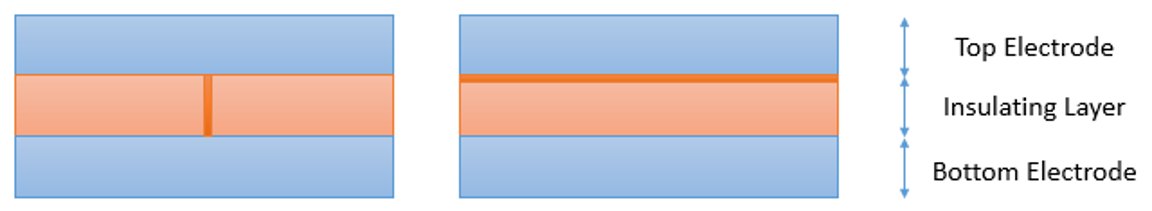
\includegraphics[width=1\textwidth]{Chapter3/Figs/t.png}
    \caption[: Conductive regions for filamentary switching and interface switching.]{: Conductive regions for filamentary switching (left) and interface switching (right).}
    \label{fig:3t}
\end{figure}

\noindent In the context of bulk silicon oxide, the formation of a conductive filament within the insulating layer typically occurs during the electroforming process. This conductive filament is generally independent of electrode size, with the switching mechanism being dominated by a single filament. The switching process instigates a minor alteration to the filament. It has been established that this is independent of the insulating layer thickness. This is due to the fact that changes in resistance usually take place in a localised region.\\

\noindent The surface switching mechanism is comparatively under-researched in comparison to filamentary switching. The conductivity of this mechanism is found to be predominantly contingent upon the dimensions of the electrode. The primary driving force behind this mechanism is the formation of a Schottky tunnel barrier across the entire electrode interface and the insulating layer. Consequently, a switching layer is formed at the interface.\\

\begin{figure}[htbp!] 
    \centering    
    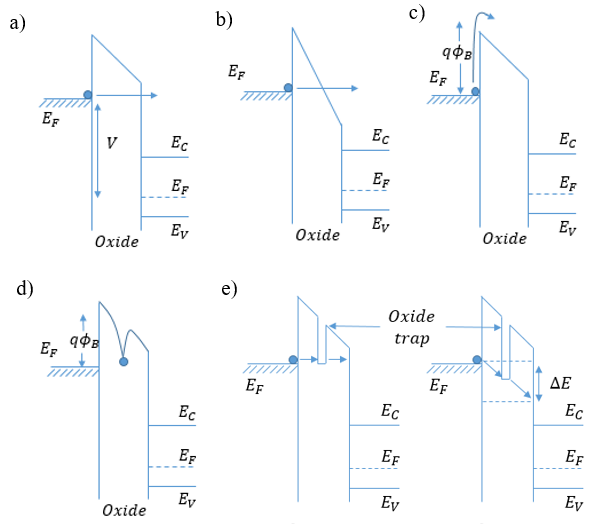
\includegraphics[width=0.65\textwidth]{Chapter3/Figs/u.png}
    \caption[Energy-band diagrams showing different conduction mechanisms.]{Energy-band diagrams showing different conduction mechanisms: (a) direct tunnelling, (b) Fowler-Nordheim tunnelling, (c) thermionic emission, (d) Poole-Frenkel emission, (e) trap-assisted tunnelling \cite{sze2021physics}}
    \label{fig:3u}
\end{figure}

\noindent Electrical conductivity is defined as an intrinsic property that determines the extent to which a given material can oppose a flow of charge. The ideal insulator is characterised by a complete absence of conductance and infinite resistance. It is evident that the conductivity of the silicon oxide thin film, which is measured in several hundred nanometres, is suboptimal due to the presence of a finite amount of conductance. The conductivity of the semiconductor material is also contingent on a variety of external conditions. The aforementioned parameters encompass specific frequencies of light, temperature dependency and applied electric field.
\begin{align}
    E = \frac{V}{d} \label{eq:3.1}
\end{align}

\noindent In  (\ref{eq:3.1}), the electric field strength, E, can be expressed as a function of the applied voltage, V, and the distance that the voltage is being applied across, d. Nevertheless, it is important to note that this fundamental estimate may not be applicable to the actual devices. The validity of assumptions regarding negligible oxide charges, voltage flat-band and small band bending may be called into question. In order to facilitate a more thorough analysis and identification of the switching procedure in the samples, additional conduction mechanisms in the insulator are considered.
\begin{align}
    J &\propto E^{2} exp\left[ -\frac{4\sqrt{2m^{*}}(q\phi _{B})^{^{3/2}}}{3q\hslash E_{i}} \right] \label{eq:3.2} \\
    J &\propto V^2exp \left( -\frac{b}{V}\right) \label{eq:3.3}
\end{align}

\noindent (\ref{eq:3.2}) displays the tunnelling current density's dependence on the electric field and voltage, applied as appropriate, while being independent of temperature. In the context of the aforementioned equation, $\phi_B$ denotes the tunnelling barrier height, E represents the insulator electric field, $m^*$ is defined as 0.42m, which is the carrier effective mass for silicon oxide, $\hslash$ is the reduced Planck constant, $q$ is the electric charge, and $b$ is a constant of proportionality.\\

\noindent In the presence of a strong electric field, conventional tunnelling is the predominant conduction mode for insulating materials. The tunnelling process is a consequence of quantum mechanical effects, with the electron wave function having a finite probability of penetrating through a potential barrier of finite height. Conventional quantum tunnelling refers to the direct passage of an electron through the entire width of a barrier. Alternatively, Fowler-Nordheim tunnelling refers to the electron tunnelling through only part of this height.
\begin{align}
    J &\propto E \cdot exp\left( -\frac{\Delta E_a}{kT} \right) \label{eq:3.4} \\
    J &\propto \frac{V}{T} \cdot exp \left( -\frac{c}{T}\right) \label{eq:3.5}
\end{align}

\noindent (\ref{eq:3.4})  illustrates the ohmic current density as a function of electric field, as well as the voltage applied and the temperature. In this equation, $\Delta E_a$ denotes the activation energy, $k$ is the Boltzmann constant, $T$ is the temperature in Kelvin and $c$ is a constant of proportionality. In the context of low fields and elevated temperatures, ohmic conduction exerts a predominant influence. This phenomenon entails the thermally induced excitation of carriers, thereby facilitating their transition between conductive states.
\begin{align}
    J &\propto \frac{E}{T} \cdot exp\left( -\frac{\Delta E_a}{kT} \right) \label{eq:3.6} \\
    J &\propto \frac{V}{T} \cdot exp \left( -\frac{d}{T}\right) \label{eq:3.7}
\end{align}
\noindent Ionic conduction exhibits a comparable expression to ohmic conduction, yet it possesses a distinct activation energy and constant of proportionality. This process is typically characterised by the movement of ions across a material via defects in the crystal lattice of a solid. For an ideal insulator, ions cannot readily travel into and out of the material. \\

\noindent However, an applied electric field will result in the build-up of ionic carriers at the metal-to-insulator interfaces, thereby modifying the voltage distribution across the region. The elimination of the applied electric field will result in the retention of a significant internal field, thereby enabling the flow of an ionic current until equilibrium is achieved.
\begin{align}
    J &= \frac{9\varepsilon _i \mu V^2}{8d^3} \label{eq:3.8} \\
    J &\propto V^2 \label{eq:3.9}
\end{align}

\noindent The phenomenon of space charge can be attributed to the injection of charge from the electrodes into the insulator, in the absence of compensating charges. The process involves the injection of charges into the dielectric from one electrode and their subsequent capture by the other. The Mott–Gurney law is delineated in (\ref{eq:3.8}) for space charge limited current in solid and in the velocity-saturation regime accordingly. \\

\noindent In this equation, $\epsilon$ denotes the dielectric permittivity, $\mu$ is the carrier mobility, $L$ is the material thickness, and $v = \mu E$ is the electron drift velocity. This conduction mechanism is predicated on the presence of a single type of charge carrier, the absence of intrinsic conductivity, and an electric field of zero magnitude at the cathode responsible for the injection of charge.\\

\noindent Further exploration will be directed towards other conduction mechanisms, including Schottky emission and Poole-Frenkel conduction, which will be examined in greater detail. Schottky emission, otherwise known as thermionic emission, occurs when the carriers receive thermal energy in excess of the potential barrier height. The phenomenon of Poole-Frenkel conduction occurs when trapped electrons are thermally excited into the conduction band.

\subsubsection[Fowler-Nordheim Tunnelling]{Fowler-Nordheim Tunnelling}

\noindent In the presence of elevated electric fields, quantum mechanical tunnelling emerges as the predominant conduction mechanism in insulating materials. This is a consequence of the process inherent in quantum mechanics, whereby the electron wave function is capable of penetrating a potential barrier. \\

\noindent This process is typically contingent on the electric field, irrespective of temperature. The phenomenon of direct tunnelling occurs when carriers traverse the entire width of the barrier. It has been established that, in the context of Fowler-Nordheim tunnelling, carriers only traverse a proportion of this width.
\begin{align}
    J &= \frac{q^2E^2}{8\pi\hslash\phi _B} exp \left[  -\frac{4\sqrt{2m^{*}}(q\phi _{B})^{^{3/2}}}{3q\hslash E_{i}} \right] \label{eq:3.10} \\
    J &\propto \frac{4\pi q m^* kT}{\hslash^3} \label{eq:3.11}
\end{align}

\noindent The phenomenon of Fowler-Nordheim tunnelling is contingent upon the trapezoidal configuration of the potential barrier. In the presence of a substantial application of an electric field, an increased incidence of band-bending is observed. This results in a significant reduction in the effective width required for carriers to tunnel through. In the context of a thick oxide layer, this is the prevailing conduction mechanism for a metal oxide structure. Subsequent to the tunnelling process, the carriers are able to move freely between the conduction and valence bands.\\

\noindent The identification of the mechanism for the device is possible through the rearrangement of (\ref{eq:3.10}) and the graphical representation of the Fowler-Nordheim plot of $ln(J/E^2)$ against $\frac{1}{E}$ for experimental I-V characterisations. The gradient of this straight-line plot is equivalent to $-\frac{4\sqrt{2m^{*}}(q\phi _{B})^{^{3/2}}}{3q\hslash}$, which can be rearranged to obtain the barrier height $\phi_B$. The y-intercept, on the other hand, describes the geometrical efficiency of electron-field emission. The occurrence of this mechanism is contingent upon the product of the electric field and layer thickness exceeding the barrier height.

\subsubsection[Poole-Frenkel Conduction Mechanism]{Poole-Frenkel Conduction Mechanism}

\noindent Conduction may also occur in the absence of quantum tunnelling through the insulator. In the context of materials characterised by a high density of structural defects, the movement of carriers is constrained in a manner that is distinct from the behaviour exhibited by tunnelling mechanisms. The presence of these structural defects also gives rise to the appearance of additional energy states, also known as traps, in the vicinity of the energy band edges. The function of these traps is to restrict the flow of current, and they achieve this by means of a capture and release process.\\

\noindent The Poole-Frenkel conduction mechanism is concerned with electrons trapped in these states. These trapped electrons can eventually amass sufficient energy via thermal fluctuations in the material to escape from the localized trap states. It is imperative to note that, in the absence of being captured in an alternative trap state, the electrons can ultimately reach the conduction band. It is evident that this mechanism is contingent on two factors: the application of an electric field and the presence of thermal energy. The electron derives its total energy from two sources: the electric field and thermal fluctuations.
\begin{align}
    J &\propto E_i \cdot exp \left[ -\frac{q(\phi _{B} - \sqrt{qE_i/\pi \varepsilon _i} )}{kT} \right] \label{eq:3.12} \\
    J &\propto V \cdot exp \left[ \frac{q}{kT} \left( 2a\sqrt{V} - \phi _{B} \right) \right] \label{eq:3.13} 
\end{align}

\noindent This conduction mechanism is typically driven by electron drift current, $J=qn\mu E$, where $q$ is the electric charge, $n$ is the carrier density, $\mu$ is the carrier mobility and $E$ is the electric field. This current may be expanded into (\ref{eq:3.12}) with dependence on the trap depth $\phi_B$, the permittivity of the insulator $\epsilon$ and the temperature $T$. A non-ideality factor $m$, varying between 1 and 2, may be introduced to the equation to account for the fabrication process and the semiconductor materials used.

\subsubsection[Thermionic Emission]{Thermionic Emission}


\subsubsection[Trap Assisted Tunnelling]{Trap Assisted Tunnelling}


\subsection[Switching Model Analysis]{Switching Model Analysis}


\section[Summary]{Summary}

